\documentclass[landscape]{article}

\usepackage[utf8]{inputenc}
\usepackage[english]{babel}

\usepackage{amsmath,amsfonts,amssymb}
\usepackage{fullpage}
\usepackage{verbatim}

\usepackage[margin=10mm, top=10mm, bottom=5mm]{geometry}

\usepackage{tikz,pgfplots}

\pgfplotsset{
  width=240mm,height=190mm,
  major grid style={thin,dotted,color=black!50},
  minor grid style={thin,dotted,color=black!50},
  grid,
  every axis/.append style={
    line width=0.5pt,
    tick style={
      line cap=round,
      thin,
      major tick length=4pt,
      minor tick length=2pt,
    },
  },
  legend cell align=left,
  legend pos=north west,
  compat=1.9
}

%%%%%%%%%%%%%%%%%%%%%%%%%%%%%%%%%%%%%%%%%%%%%%%%%%%%%%%%%%%%%%%%%%%%%%%%%%%%%%%%

\begin{document}

% IMPORT-DATA ResultsQS ResultsQS_muc.txt

%%%%%%%%%%%%%%%%%%%%%%%%%%%%%%%%%%%%%%%%%%%%%%%%%%%%%%%%%%%%%%%%%%%%%%%%%%%%%%%%

\begin{center}

\begin{tikzpicture}
  \begin{axis}[
    title={MPI, $2^{13}$ Cores},
    xlabel={Elements [$\log_2(n)$]},
    ylabel={Run Time / Elements [$\log_2(n)$]},
    ]   
	%% MULTIPLOT(Type) SELECT size, collective, LOG(2,elements) AS x, LOG(2,Time/elements) as y, MULTIPLOT FROM (    
	%% SELECT elements, size, MEDIAN(pivot + calculate + create_comms) as Time, 'Pivot + Prefix + CreateComms' as Type, collective, blocking, mpi_split
	%% FROM ResultsQS
	%% GROUP BY collective, size, elements, blocking, mpi_split
	%% UNION ALL
	%% SELECT elements, size, MEDIAN(partition + exchange + sort_two + sort_local) as Time, 'Partition + Exchange + SortOnTwo + SortLocal' as Type, collective, blocking, mpi_split
	%% FROM ResultsQS
	%% GROUP BY collective, size, elements, blocking, mpi_split
	%% ) a
	%% WHERE collective="mpi" AND size=8192 AND blocking=0 AND mpi_split=1
	%% GROUP BY MULTIPLOT, x  ORDER BY MULTIPLOT, x
 \addplot coordinates { (0.0,-11.4447) (1.0,-10.0615) (2.0,-11.038) (3.0,-9.92395) (4.0,-11.5795) (5.0,-12.1621) (6.0,-13.538) (7.0,-13.4959) (8.0,-15.4083) (9.0,-14.6463) (10.0,-16.7165) (11.0,-16.6362) (12.0,-17.2424) (13.0,-18.7553) (14.0,-17.3575) (15.0,-17.6043) (16.0,-18.3013) (17.0,-18.8636) (18.0,-19.3048) (19.0,-19.4083) (20.0,-19.3005) };
 \addlegendentry{Type=Partition + Exchange + SortOnTwo + SortLocal};
 \addplot coordinates { (0.0,-2.0936) (1.0,-2.84868) (2.0,-3.26651) (3.0,-4.21624) (4.0,-5.65592) (5.0,-6.47171) (6.0,-7.54659) (7.0,-8.18518) (8.0,-9.38782) (9.0,-9.84959) (10.0,-11.2444) (11.0,-11.9578) (12.0,-13.3246) (13.0,-14.483) (14.0,-14.9353) (15.0,-15.8995) (16.0,-16.96) (17.0,-18.0167) (18.0,-19.0767) (19.0,-19.8358) (20.0,-20.227) };
 \addlegendentry{Type=Pivot + Prefix + CreateComms};


  \end{axis}
\end{tikzpicture}
\newpage

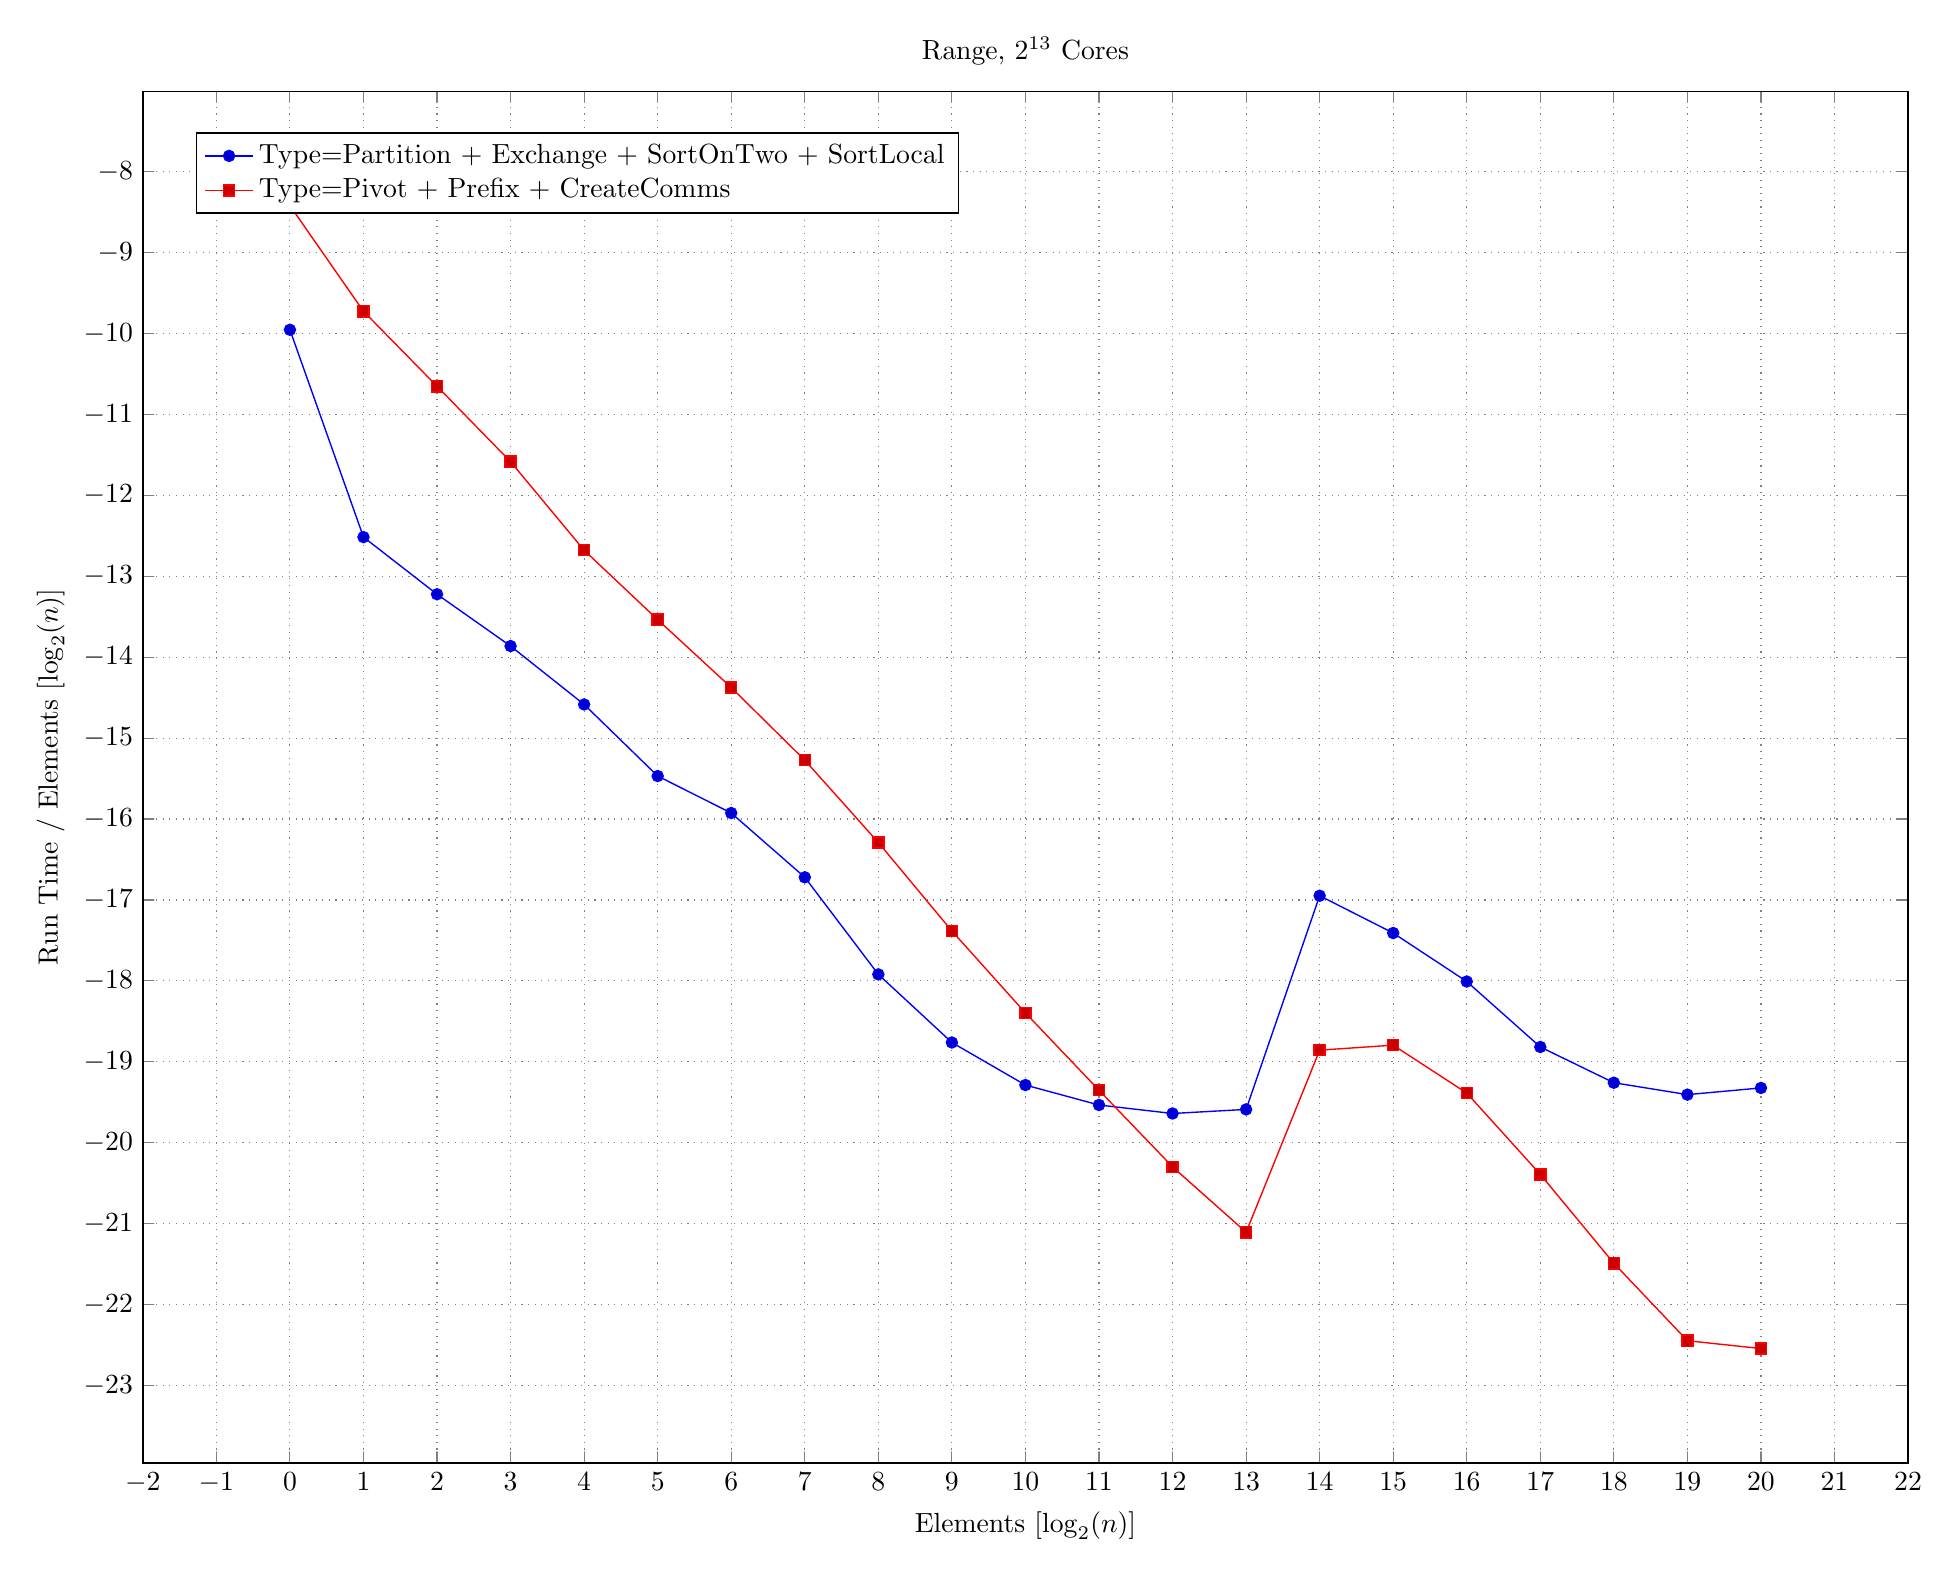
\begin{tikzpicture}
  \begin{axis}[
    title={Range, $2^{13}$ Cores},
    xlabel={Elements [$\log_2(n)$]},
    ylabel={Run Time / Elements [$\log_2(n)$]},
    ]   
	%% MULTIPLOT(Type) SELECT size, collective, LOG(2,elements) AS x, LOG(2,Time/elements) as y, MULTIPLOT FROM (    
	%% SELECT elements, size, MEDIAN(pivot + calculate + create_comms) as Time, 'Pivot + Prefix + CreateComms' as Type, collective, blocking, mpi_split
	%% FROM ResultsQS
	%% GROUP BY collective, size, elements, blocking, mpi_split
	%% UNION ALL
	%% SELECT elements, size, MEDIAN(partition + exchange + sort_two + sort_local) as Time, 'Partition + Exchange + SortOnTwo + SortLocal' as Type, collective, blocking, mpi_split
	%% FROM ResultsQS
	%% GROUP BY collective, size, elements, blocking, mpi_split
	%% ) a
	%% WHERE collective="range" AND size=8192 AND blocking=0 AND mpi_split=0 
	%% GROUP BY MULTIPLOT, x  ORDER BY MULTIPLOT, x
 \addplot coordinates { (0.0,-9.95666) (1.0,-12.5176) (2.0,-13.2237) (3.0,-13.8637) (4.0,-14.5849) (5.0,-15.469) (6.0,-15.9259) (7.0,-16.7196) (8.0,-17.919) (9.0,-18.7604) (10.0,-19.286) (11.0,-19.5325) (12.0,-19.6371) (13.0,-19.5869) (14.0,-16.9474) (15.0,-17.4081) (16.0,-18.0072) (17.0,-18.8156) (18.0,-19.2572) (19.0,-19.4042) (20.0,-19.3215) };
 \addlegendentry{Type=Partition + Exchange + SortOnTwo + SortLocal};
 \addplot coordinates { (0.0,-8.423) (1.0,-9.72858) (2.0,-10.6546) (3.0,-11.5863) (4.0,-12.6803) (5.0,-13.5376) (6.0,-14.376) (7.0,-15.2729) (8.0,-16.2901) (9.0,-17.3829) (10.0,-18.395) (11.0,-19.3498) (12.0,-20.2965) (13.0,-21.1045) (14.0,-18.8549) (15.0,-18.7933) (16.0,-19.3847) (17.0,-20.3893) (18.0,-21.4875) (19.0,-22.4439) (20.0,-22.5407) };
 \addlegendentry{Type=Pivot + Prefix + CreateComms};


  \end{axis}
\end{tikzpicture}
\newpage

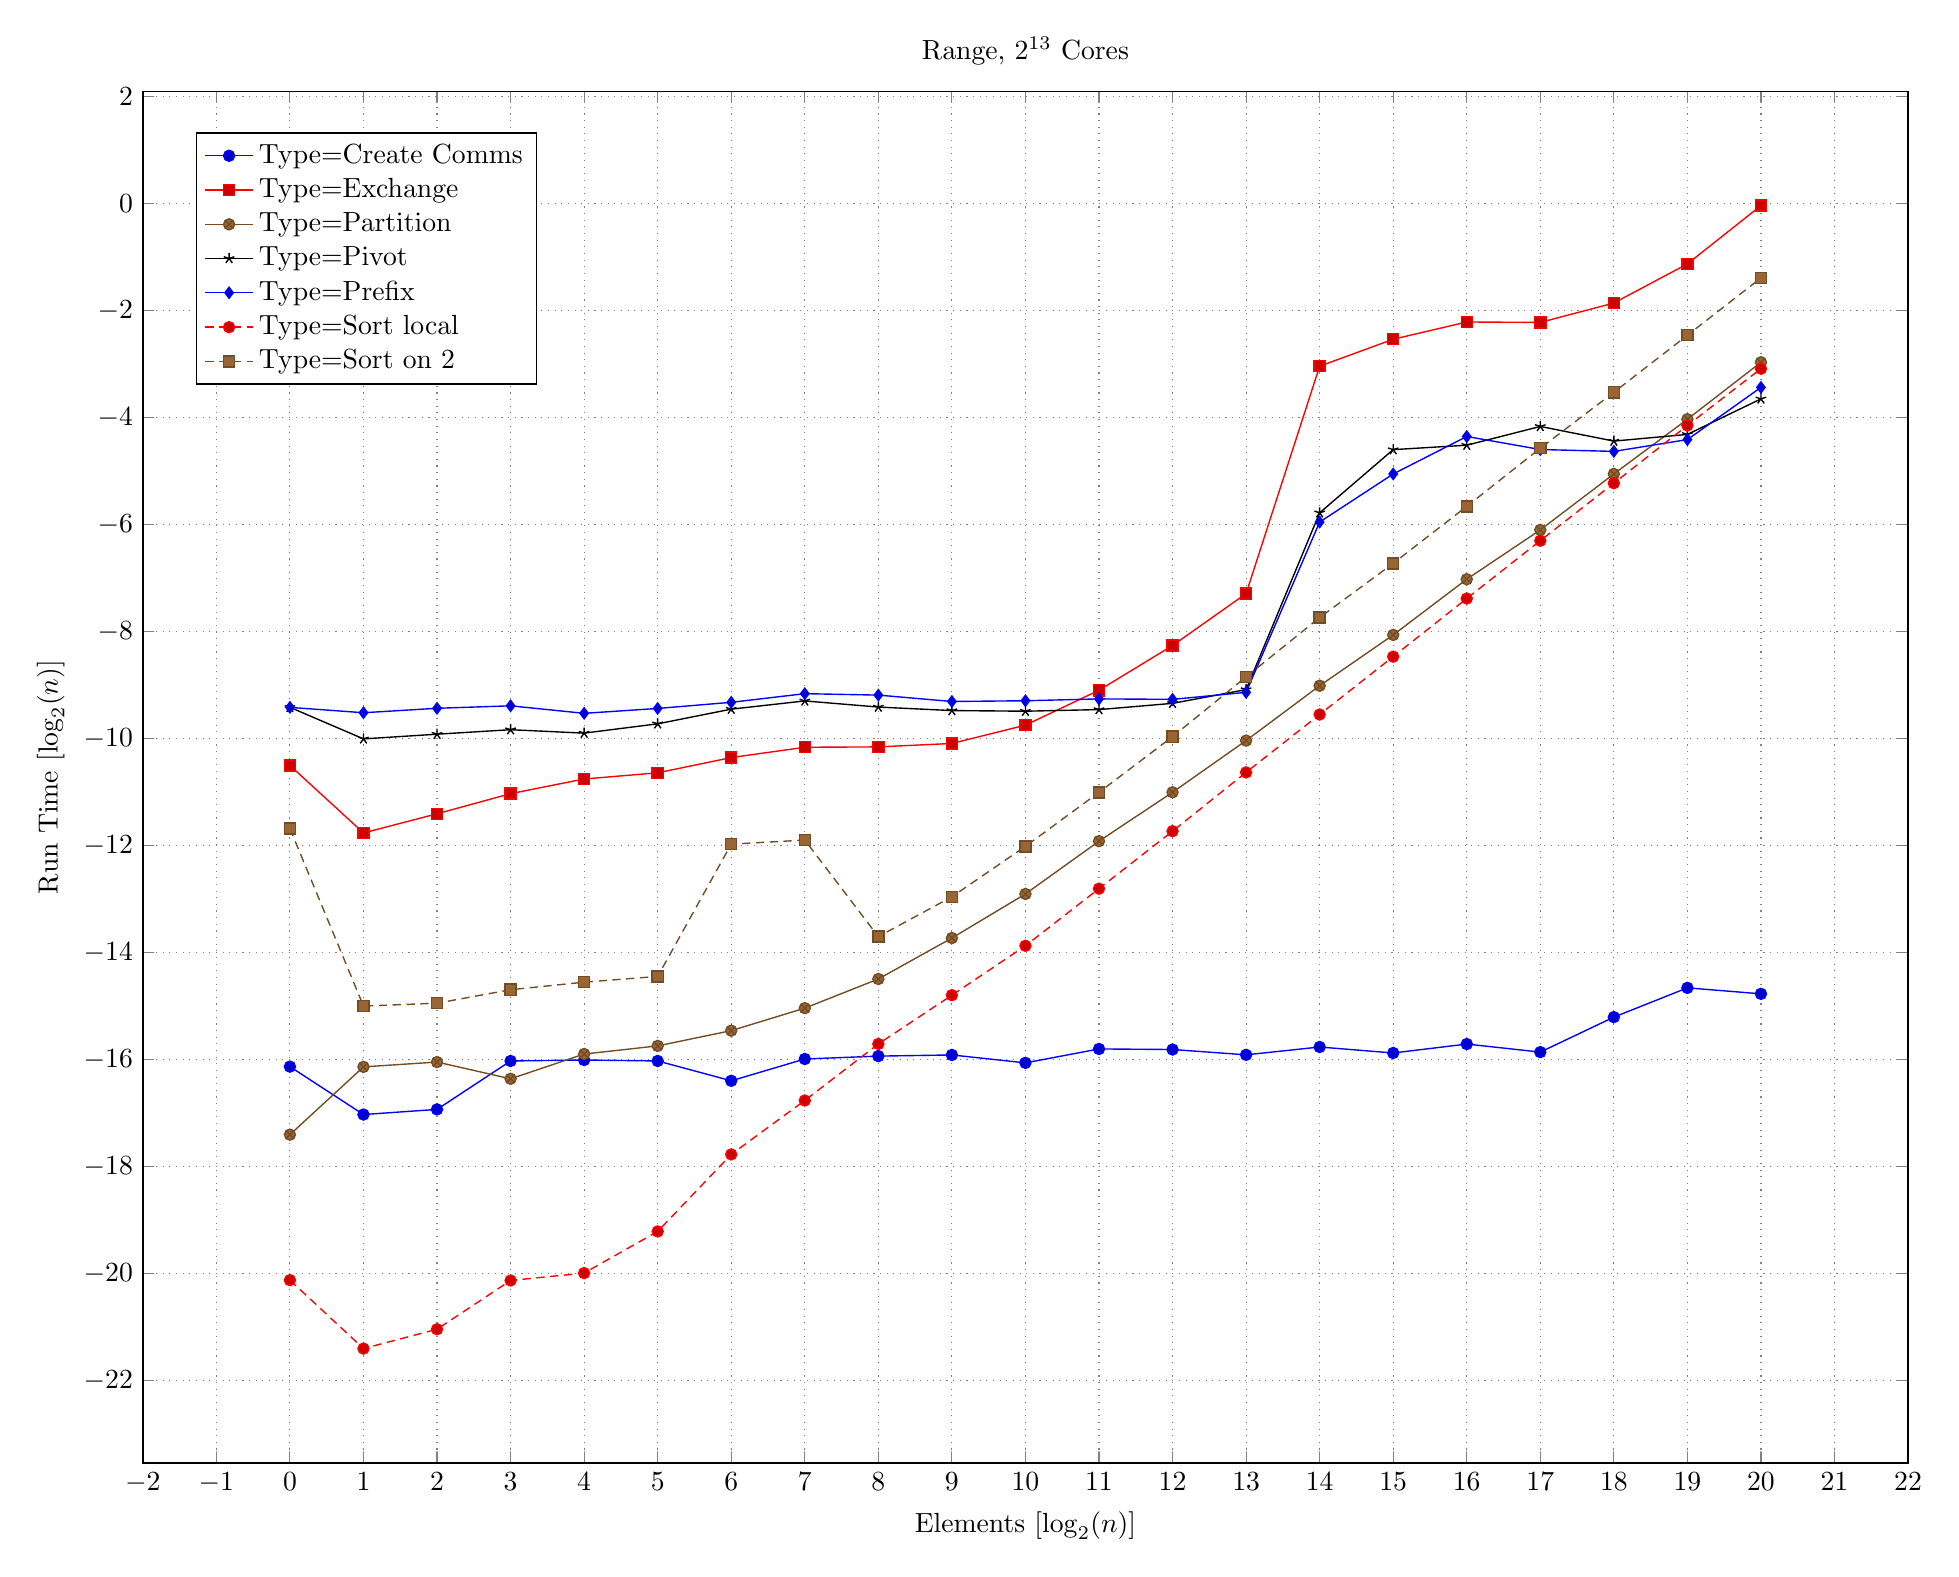
\begin{tikzpicture}
  \begin{axis}[
    title={Range, $2^{13}$ Cores},
    xlabel={Elements [$\log_2(n)$]},
    ylabel={Run Time [$\log_2(n)$]},
    ]   
	%% MULTIPLOT(Type) SELECT size, collective, LOG(2,elements) AS x, LOG(2,Time) as y, MULTIPLOT FROM (    
	%% SELECT elements, size, MEDIAN(pivot) as Time, 'Pivot' as Type, collective, blocking, mpi_split
	%% FROM ResultsQS
	%% GROUP BY collective, size, elements, blocking, mpi_split
	%% UNION ALL
	%% SELECT elements, size, MEDIAN(partition) as Time, 'Partition' as Type, collective, blocking, mpi_split
	%% FROM ResultsQS
	%% GROUP BY collective, size, elements, blocking, mpi_split
	%% UNION ALL
	%% SELECT elements, size, MEDIAN(calculate) as Time, 'Prefix' as Type, collective, blocking, mpi_split
	%% FROM ResultsQS
	%% GROUP BY collective, size, elements, blocking, mpi_split
	%% UNION ALL
	%% SELECT elements, size, MEDIAN(exchange) as Time, 'Exchange' as Type, collective, blocking, mpi_split
	%% FROM ResultsQS
	%% GROUP BY collective, size, elements, blocking, mpi_split
	%% UNION ALL
	%% SELECT elements, size, MEDIAN(create_comms) as Time, 'Create Comms' as Type, collective, blocking, mpi_split
	%% FROM ResultsQS
	%% GROUP BY collective, size, elements, blocking, mpi_split
	%% UNION ALL
	%% SELECT elements, size, MEDIAN(sort_two) as Time, 'Sort on 2' as Type, collective, blocking, mpi_split
	%% FROM ResultsQS
	%% GROUP BY collective, size, elements, blocking, mpi_split
	%% UNION ALL
	%% SELECT elements, size, MEDIAN(sort_local) as Time, 'Sort local' as Type, collective, blocking, mpi_split
	%% FROM ResultsQS
	%% GROUP BY collective, size, elements, blocking, mpi_split
	%% ) a
	%% WHERE collective="range" AND size=8192 AND blocking=0 AND mpi_split=0
	%% GROUP BY MULTIPLOT, x  ORDER BY MULTIPLOT, x
 \addplot coordinates { (0.0,-16.1337) (1.0,-17.0292) (2.0,-16.9332) (3.0,-16.0283) (4.0,-16.0097) (5.0,-16.0278) (6.0,-16.3987) (7.0,-15.9909) (8.0,-15.9372) (9.0,-15.9155) (10.0,-16.0634) (11.0,-15.8032) (12.0,-15.8139) (13.0,-15.9129) (14.0,-15.7669) (15.0,-15.8788) (16.0,-15.7117) (17.0,-15.8623) (18.0,-15.2083) (19.0,-14.6611) (20.0,-14.7729) };
 \addlegendentry{Type=Create Comms};
 \addplot coordinates { (0.0,-10.5033) (1.0,-11.7654) (2.0,-11.4073) (3.0,-11.0308) (4.0,-10.7571) (5.0,-10.6412) (6.0,-10.3565) (7.0,-10.1639) (8.0,-10.157) (9.0,-10.0929) (10.0,-9.7506) (11.0,-9.09873) (12.0,-8.26225) (13.0,-7.29175) (14.0,-3.04094) (15.0,-2.53665) (16.0,-2.21422) (17.0,-2.22216) (18.0,-1.86005) (19.0,-1.12836) (20.0,-0.0387879) };
 \addlegendentry{Type=Exchange};
 \addplot coordinates { (0.0,-17.4052) (1.0,-16.1385) (2.0,-16.0481) (3.0,-16.3613) (4.0,-15.8982) (5.0,-15.7462) (6.0,-15.4608) (7.0,-15.0405) (8.0,-14.4955) (9.0,-13.73) (10.0,-12.9057) (11.0,-11.9192) (12.0,-11.0056) (13.0,-10.0389) (14.0,-9.01366) (15.0,-8.06408) (16.0,-7.02289) (17.0,-6.10139) (18.0,-5.05477) (19.0,-4.03194) (20.0,-2.96709) };
 \addlegendentry{Type=Partition};
 \addplot coordinates { (0.0,-9.41715) (1.0,-10.0073) (2.0,-9.91977) (3.0,-9.83553) (4.0,-9.89983) (5.0,-9.72557) (6.0,-9.45166) (7.0,-9.29764) (8.0,-9.41241) (9.0,-9.47791) (10.0,-9.48986) (11.0,-9.45965) (12.0,-9.34309) (13.0,-9.08593) (14.0,-5.78171) (15.0,-4.60033) (16.0,-4.51737) (17.0,-4.16693) (18.0,-4.44051) (19.0,-4.31631) (20.0,-3.65149) };
 \addlegendentry{Type=Pivot};
 \addplot coordinates { (0.0,-9.41822) (1.0,-9.51839) (2.0,-9.43508) (3.0,-9.38911) (4.0,-9.52951) (5.0,-9.43822) (6.0,-9.32369) (7.0,-9.16218) (8.0,-9.18883) (9.0,-9.30819) (10.0,-9.29451) (11.0,-9.25987) (12.0,-9.26811) (13.0,-9.13754) (14.0,-5.95375) (15.0,-5.05524) (16.0,-4.35452) (17.0,-4.59825) (18.0,-4.63313) (19.0,-4.41266) (20.0,-3.43686) };
 \addlegendentry{Type=Prefix};
 \addplot coordinates { (0.0,-20.125) (1.0,-21.4038) (2.0,-21.0429) (3.0,-20.1312) (4.0,-19.993) (5.0,-19.2145) (6.0,-17.7748) (7.0,-16.7668) (8.0,-15.7098) (9.0,-14.7985) (10.0,-13.8747) (11.0,-12.807) (12.0,-11.7327) (13.0,-10.6335) (14.0,-9.55172) (15.0,-8.46995) (16.0,-7.38346) (17.0,-6.30249) (18.0,-5.22782) (19.0,-4.14857) (20.0,-3.08769) };
 \addlegendentry{Type=Sort local};
 \addplot coordinates { (0.0,-11.6833) (1.0,-15.002) (2.0,-14.948) (3.0,-14.6961) (4.0,-14.5551) (5.0,-14.4474) (6.0,-11.9752) (7.0,-11.8985) (8.0,-13.7034) (9.0,-12.9592) (10.0,-12.0162) (11.0,-11.0068) (12.0,-9.96585) (13.0,-8.848) (14.0,-7.73951) (15.0,-6.72616) (16.0,-5.66095) (17.0,-4.57393) (18.0,-3.52863) (19.0,-2.46237) (20.0,-1.39038) };
 \addlegendentry{Type=Sort on 2};


  \end{axis}
\end{tikzpicture}
\newpage

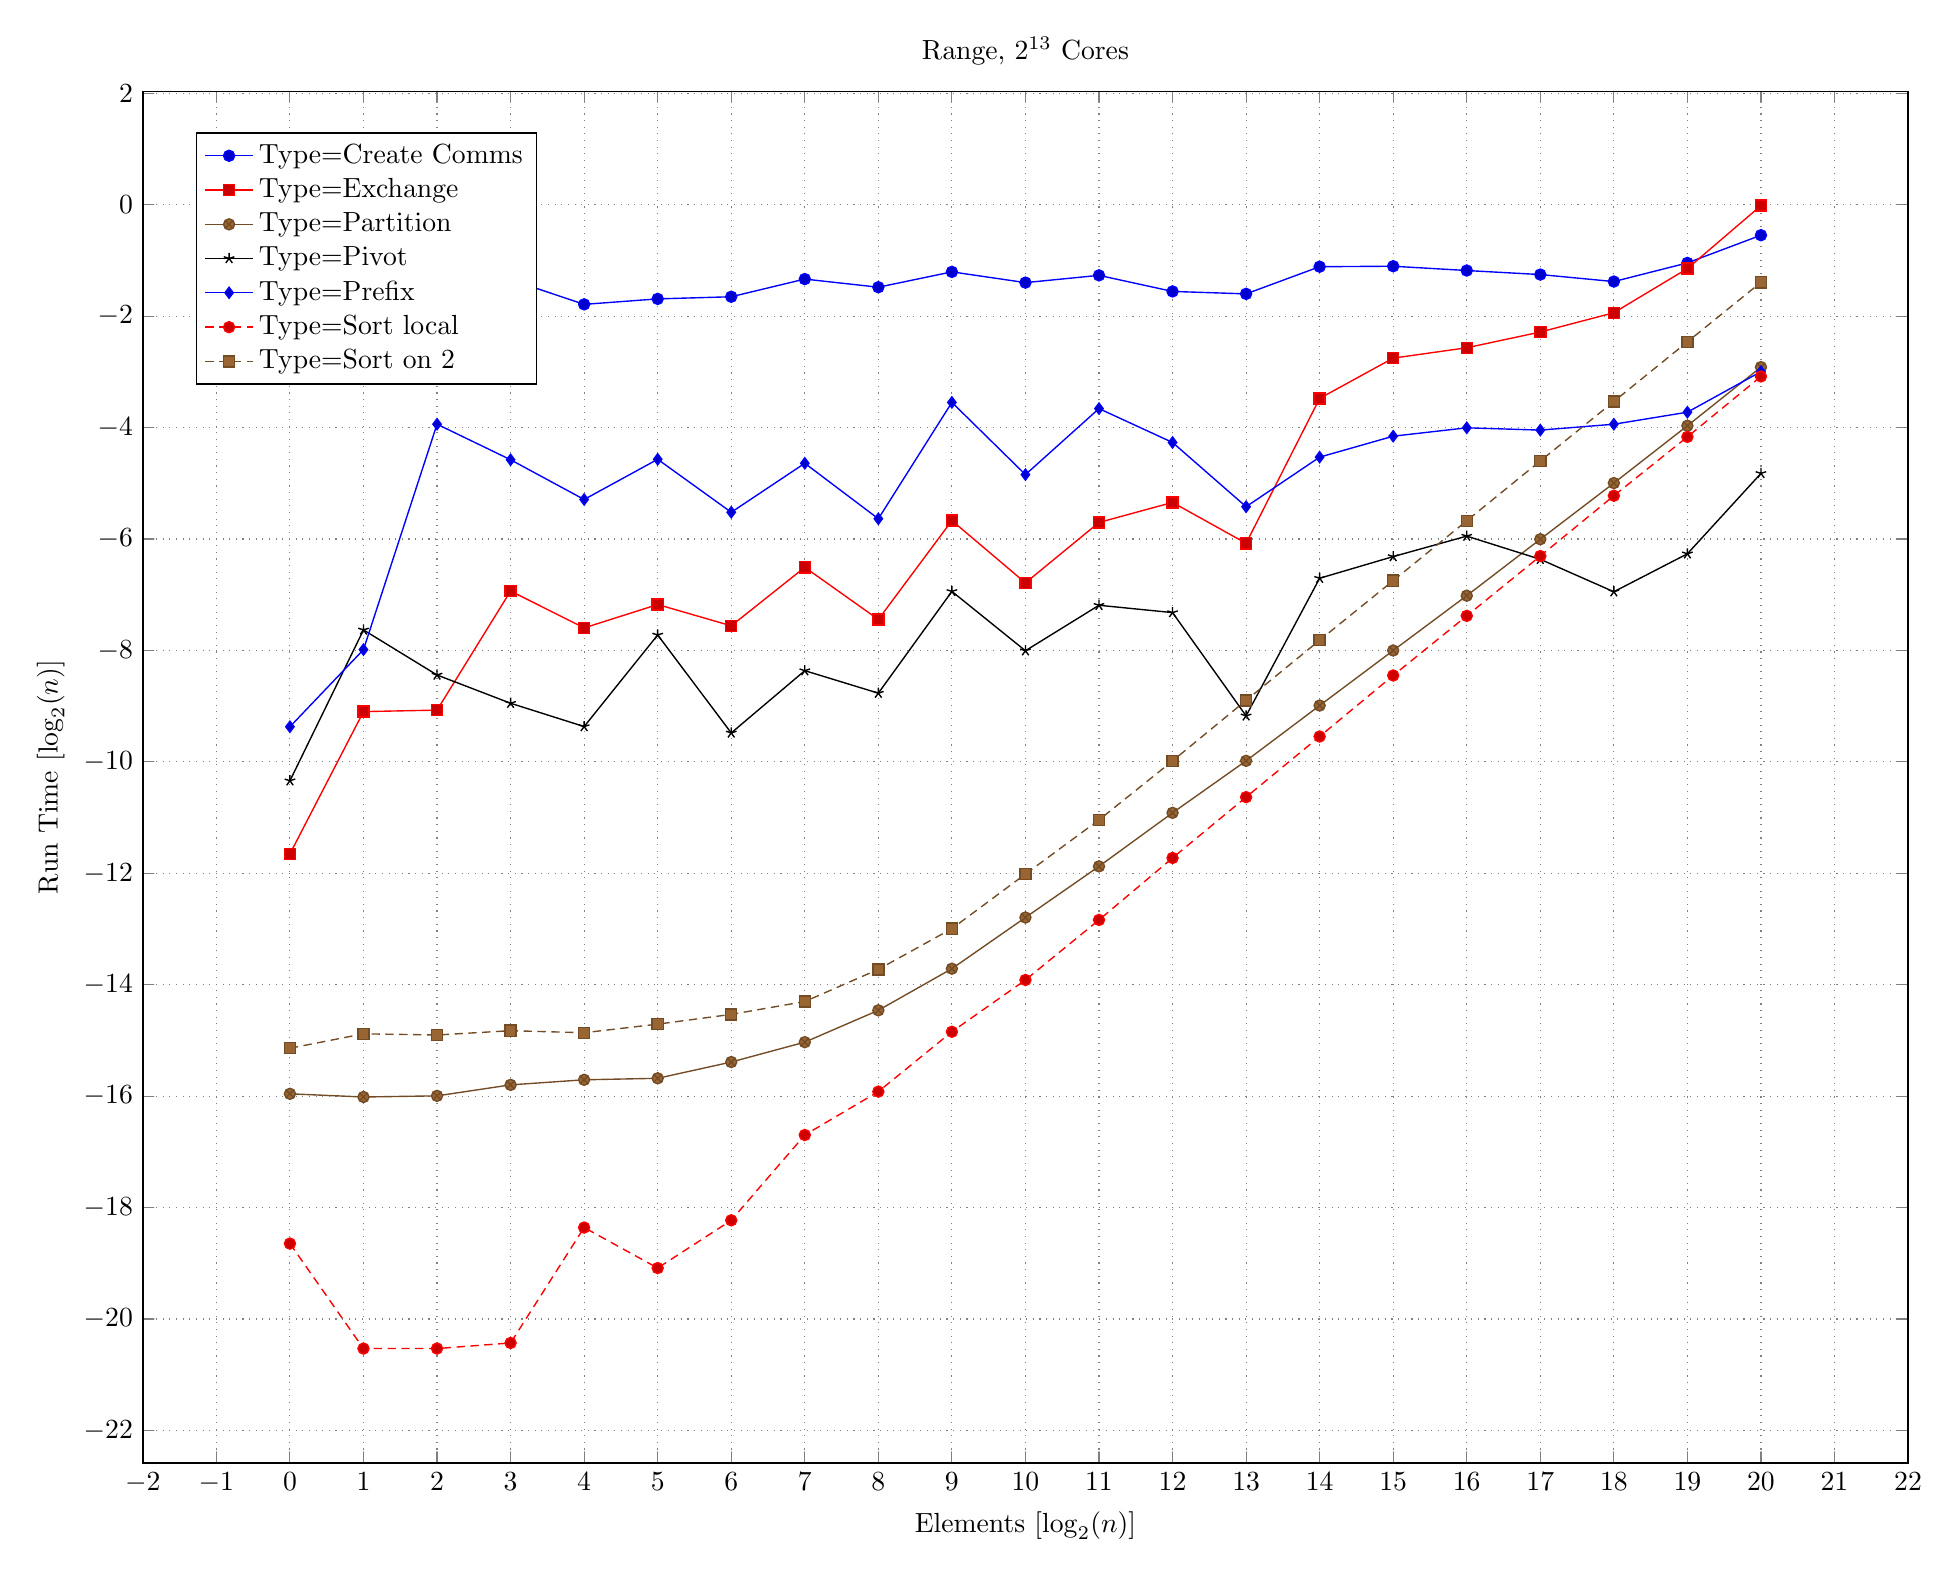
\begin{tikzpicture}
  \begin{axis}[
    title={Range, $2^{13}$ Cores},
    xlabel={Elements [$\log_2(n)$]},
    ylabel={Run Time [$\log_2(n)$]},
    ]   
	%% MULTIPLOT(Type) SELECT size, collective, LOG(2,elements) AS x, LOG(2,Time) as y, MULTIPLOT FROM (    
	%% SELECT elements, size, MEDIAN(pivot) as Time, 'Pivot' as Type, collective, blocking, mpi_split
	%% FROM ResultsQS
	%% GROUP BY collective, size, elements, blocking, mpi_split
	%% UNION ALL
	%% SELECT elements, size, MEDIAN(partition) as Time, 'Partition' as Type, collective, blocking, mpi_split
	%% FROM ResultsQS
	%% GROUP BY collective, size, elements, blocking, mpi_split
	%% UNION ALL
	%% SELECT elements, size, MEDIAN(calculate) as Time, 'Prefix' as Type, collective, blocking, mpi_split
	%% FROM ResultsQS
	%% GROUP BY collective, size, elements, blocking, mpi_split
	%% UNION ALL
	%% SELECT elements, size, MEDIAN(exchange) as Time, 'Exchange' as Type, collective, blocking, mpi_split
	%% FROM ResultsQS
	%% GROUP BY collective, size, elements, blocking, mpi_split
	%% UNION ALL
	%% SELECT elements, size, MEDIAN(create_comms) as Time, 'Create Comms' as Type, collective, blocking, mpi_split
	%% FROM ResultsQS
	%% GROUP BY collective, size, elements, blocking, mpi_split
	%% UNION ALL
	%% SELECT elements, size, MEDIAN(sort_two) as Time, 'Sort on 2' as Type, collective, blocking, mpi_split
	%% FROM ResultsQS
	%% GROUP BY collective, size, elements, blocking, mpi_split
	%% UNION ALL
	%% SELECT elements, size, MEDIAN(sort_local) as Time, 'Sort local' as Type, collective, blocking, mpi_split
	%% FROM ResultsQS
	%% GROUP BY collective, size, elements, blocking, mpi_split
	%% ) a
	%% WHERE collective="mpi" AND size=8192 AND blocking=0 AND mpi_split=1
	%% GROUP BY MULTIPLOT, x  ORDER BY MULTIPLOT, x
 \addplot coordinates { (0.0,-2.10953) (1.0,-1.89524) (2.0,-1.54366) (3.0,-1.34484) (4.0,-1.78848) (5.0,-1.69025) (6.0,-1.65204) (7.0,-1.3347) (8.0,-1.48076) (9.0,-1.20522) (10.0,-1.39828) (11.0,-1.26784) (12.0,-1.55654) (13.0,-1.60013) (14.0,-1.11254) (15.0,-1.10409) (16.0,-1.18116) (17.0,-1.25349) (18.0,-1.37938) (19.0,-1.04438) (20.0,-0.547308) };
 \addlegendentry{Type=Create Comms};
 \addplot coordinates { (0.0,-11.6519) (1.0,-9.0982) (2.0,-9.07142) (3.0,-6.93369) (4.0,-7.59571) (5.0,-7.17585) (6.0,-7.55844) (7.0,-6.50802) (8.0,-7.44411) (9.0,-5.66937) (10.0,-6.78742) (11.0,-5.70274) (12.0,-5.34335) (13.0,-6.07781) (14.0,-3.47627) (15.0,-2.75324) (16.0,-2.56747) (17.0,-2.28503) (18.0,-1.93877) (19.0,-1.14596) (20.0,-0.01604) };
 \addlegendentry{Type=Exchange};
 \addplot coordinates { (0.0,-15.9582) (1.0,-16.0153) (2.0,-15.9948) (3.0,-15.7976) (4.0,-15.7065) (5.0,-15.6797) (6.0,-15.3877) (7.0,-15.031) (8.0,-14.4596) (9.0,-13.7123) (10.0,-12.7938) (11.0,-11.8756) (12.0,-10.915) (13.0,-9.98134) (14.0,-8.98894) (15.0,-8.00101) (16.0,-7.01726) (17.0,-6.00418) (18.0,-4.99653) (19.0,-3.96699) (20.0,-2.91486) };
 \addlegendentry{Type=Partition};
 \addplot coordinates { (0.0,-10.3393) (1.0,-7.63193) (2.0,-8.44077) (3.0,-8.94826) (4.0,-9.36652) (5.0,-7.72262) (6.0,-9.48088) (7.0,-8.36316) (8.0,-8.76699) (9.0,-6.94078) (10.0,-8.00561) (11.0,-7.18948) (12.0,-7.32101) (13.0,-9.17426) (14.0,-6.70438) (15.0,-6.31567) (16.0,-5.94824) (17.0,-6.36459) (18.0,-6.94692) (19.0,-6.26548) (20.0,-4.82258) };
 \addlegendentry{Type=Pivot};
 \addplot coordinates { (0.0,-9.36973) (1.0,-7.98516) (2.0,-3.93913) (3.0,-4.57773) (4.0,-5.29076) (5.0,-4.56948) (6.0,-5.5199) (7.0,-4.64077) (8.0,-5.63683) (9.0,-3.54787) (10.0,-4.84451) (11.0,-3.65948) (12.0,-4.26737) (13.0,-5.42029) (14.0,-4.53085) (15.0,-4.15474) (16.0,-4.00432) (17.0,-4.04538) (18.0,-3.93995) (19.0,-3.72395) (20.0,-2.99587) };
 \addlegendentry{Type=Prefix};
 \addplot coordinates { (0.0,-18.6463) (1.0,-20.5304) (2.0,-20.5304) (3.0,-20.4301) (4.0,-18.3584) (5.0,-19.0856) (6.0,-18.2285) (7.0,-16.6975) (8.0,-15.9186) (9.0,-14.8442) (10.0,-13.9152) (11.0,-12.8369) (12.0,-11.7249) (13.0,-10.6332) (14.0,-9.5447) (15.0,-8.44955) (16.0,-7.37948) (17.0,-6.30595) (18.0,-5.2236) (19.0,-4.16694) (20.0,-3.08241) };
 \addlegendentry{Type=Sort local};
 \addplot coordinates { (0.0,-15.1406) (1.0,-14.8813) (2.0,-14.9025) (3.0,-14.8251) (4.0,-14.8618) (5.0,-14.7076) (6.0,-14.5326) (7.0,-14.3022) (8.0,-13.7243) (9.0,-12.9941) (10.0,-12.0135) (11.0,-11.0421) (12.0,-9.98313) (13.0,-8.89601) (14.0,-7.81664) (15.0,-6.74775) (16.0,-5.6723) (17.0,-4.59907) (18.0,-3.53201) (19.0,-2.46114) (20.0,-1.39265) };
 \addlegendentry{Type=Sort on 2};


  \end{axis}
\end{tikzpicture}
\newpage

\begin{tikzpicture}
  \begin{axis}[
    title={MPI CreateComms, $2^{13}$ Cores},
    xlabel={Elements [$\log_2(n)$]},
    ylabel={Run Time},
    ]   
	%% MULTIPLOT(Type) SELECT size, collective, LOG(2,elements) AS x, Time as y, MULTIPLOT FROM (  
	%% SELECT elements, size, MEDIAN(create_comms) as Time, 'Create Comms' as Type, collective, blocking, mpi_split
	%% FROM ResultsQS
	%% GROUP BY collective, size, elements, blocking, mpi_split
	%% UNION ALL
	%% SELECT elements, size, MEDIAN(sum - create_comms) as Time, 'Sum - Create Comms' as Type, collective, blocking, mpi_split
	%% FROM ResultsQS
	%% GROUP BY collective, size, elements, blocking, mpi_split
	%% ) a
	%% WHERE collective="mpi" AND size=8192 AND blocking=0 AND mpi_split=1
	%% GROUP BY MULTIPLOT, x  ORDER BY MULTIPLOT, x
 \addplot coordinates { (0.0,0.231723) (1.0,0.268829) (2.0,0.343014) (3.0,0.393697) (4.0,0.289477) (5.0,0.309874) (6.0,0.318189) (7.0,0.396473) (8.0,0.358299) (9.0,0.433704) (10.0,0.379381) (11.0,0.415282) (12.0,0.339965) (13.0,0.329848) (14.0,0.46248) (15.0,0.465195) (16.0,0.440997) (17.0,0.419432) (18.0,0.384385) (19.0,0.484853) (20.0,0.684296) };
 \addlegendentry{Type=Create Comms};
 \addplot coordinates { (0.0,0.0026345) (1.0,0.0103745) (2.0,0.073264) (3.0,0.0542575) (4.0,0.0345185) (5.0,0.0636945) (6.0,0.03012) (7.0,0.0562885) (8.0,0.0290885) (9.0,0.113258) (10.0,0.050167) (11.0,0.112402) (12.0,0.07821) (13.0,0.048309) (14.0,0.155642) (15.0,0.229704) (16.0,0.282018) (17.0,0.342383) (18.0,0.493169) (19.0,0.834943) (20.0,1.787505) };
 \addlegendentry{Type=Sum - Create Comms};


  \end{axis}
\end{tikzpicture}
\newpage

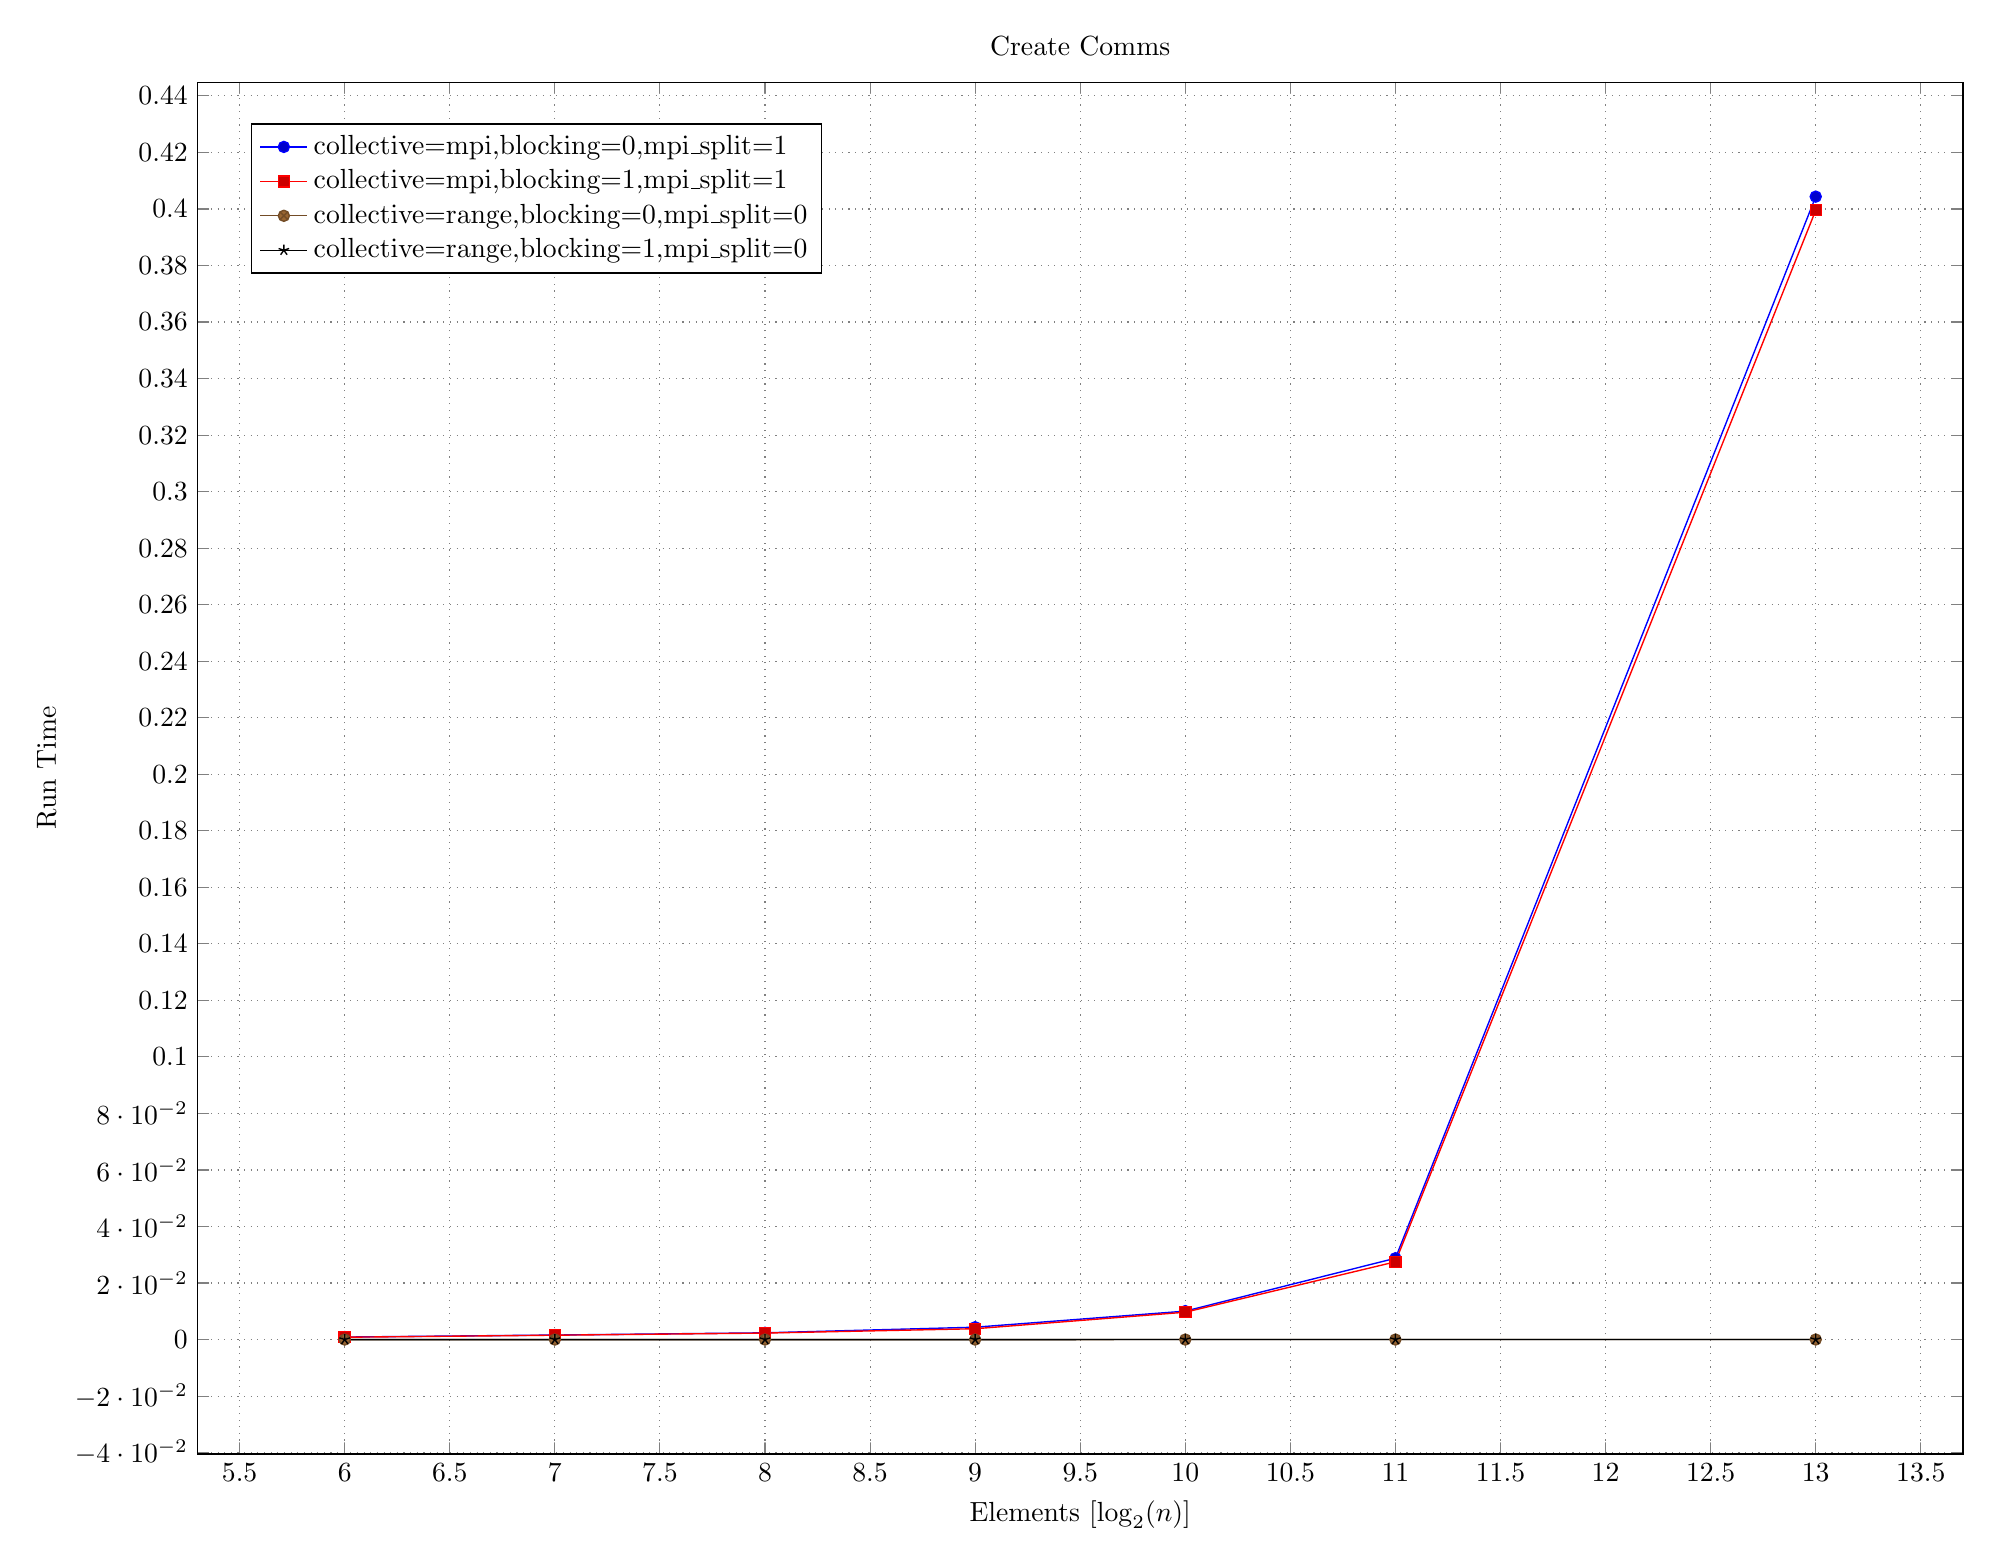
\begin{tikzpicture}
  \begin{axis}[
    title={Create Comms},
    xlabel={Elements [$\log_2(n)$]},
    ylabel={Run Time},
    ]   
	%% MULTIPLOT(collective, blocking, mpi_split) SELECT LOG(2,size) AS x, MEDIAN(create_comms) as y, MULTIPLOT
	%% FROM ResultsQS
	%% WHERE elements>POWER(2,5) AND elements<POWER(2,20)
	%% GROUP BY MULTIPLOT, x  ORDER BY MULTIPLOT, x
 \addplot coordinates { (6.0,0.000890554) (7.0,0.00160122) (8.0,0.00239009) (9.0,0.00437136) (10.0,0.0100629) (11.0,0.0287756) (13.0,0.404374) };
 \addlegendentry{collective=mpi,blocking=0,mpi\_split=1};
 \addplot coordinates { (6.0,0.000827072) (7.0,0.00154185) (8.0,0.00229749) (9.0,0.00383059) (10.0,0.00967467) (11.0,0.0275054) (13.0,0.399556) };
 \addlegendentry{collective=mpi,blocking=1,mpi\_split=1};
 \addplot coordinates { (6.0,1.46962e-06) (7.0,1.68104e-06) (8.0,1.85706e-06) (9.0,2.09734e-06) (10.0,2.61888e-06) (11.0,7.65361e-06) (13.0,1.66408e-05) };
 \addlegendentry{collective=range,blocking=0,mpi\_split=0};
 \addplot coordinates { (6.0,1.37184e-06) (7.0,1.75647e-06) (8.0,1.80677e-06) (9.0,2.07778e-06) (10.0,2.83215e-06) (11.0,7.255e-06) (13.0,1.63718e-05) };
 \addlegendentry{collective=range,blocking=1,mpi\_split=0};


  \end{axis}
\end{tikzpicture}
\newpage

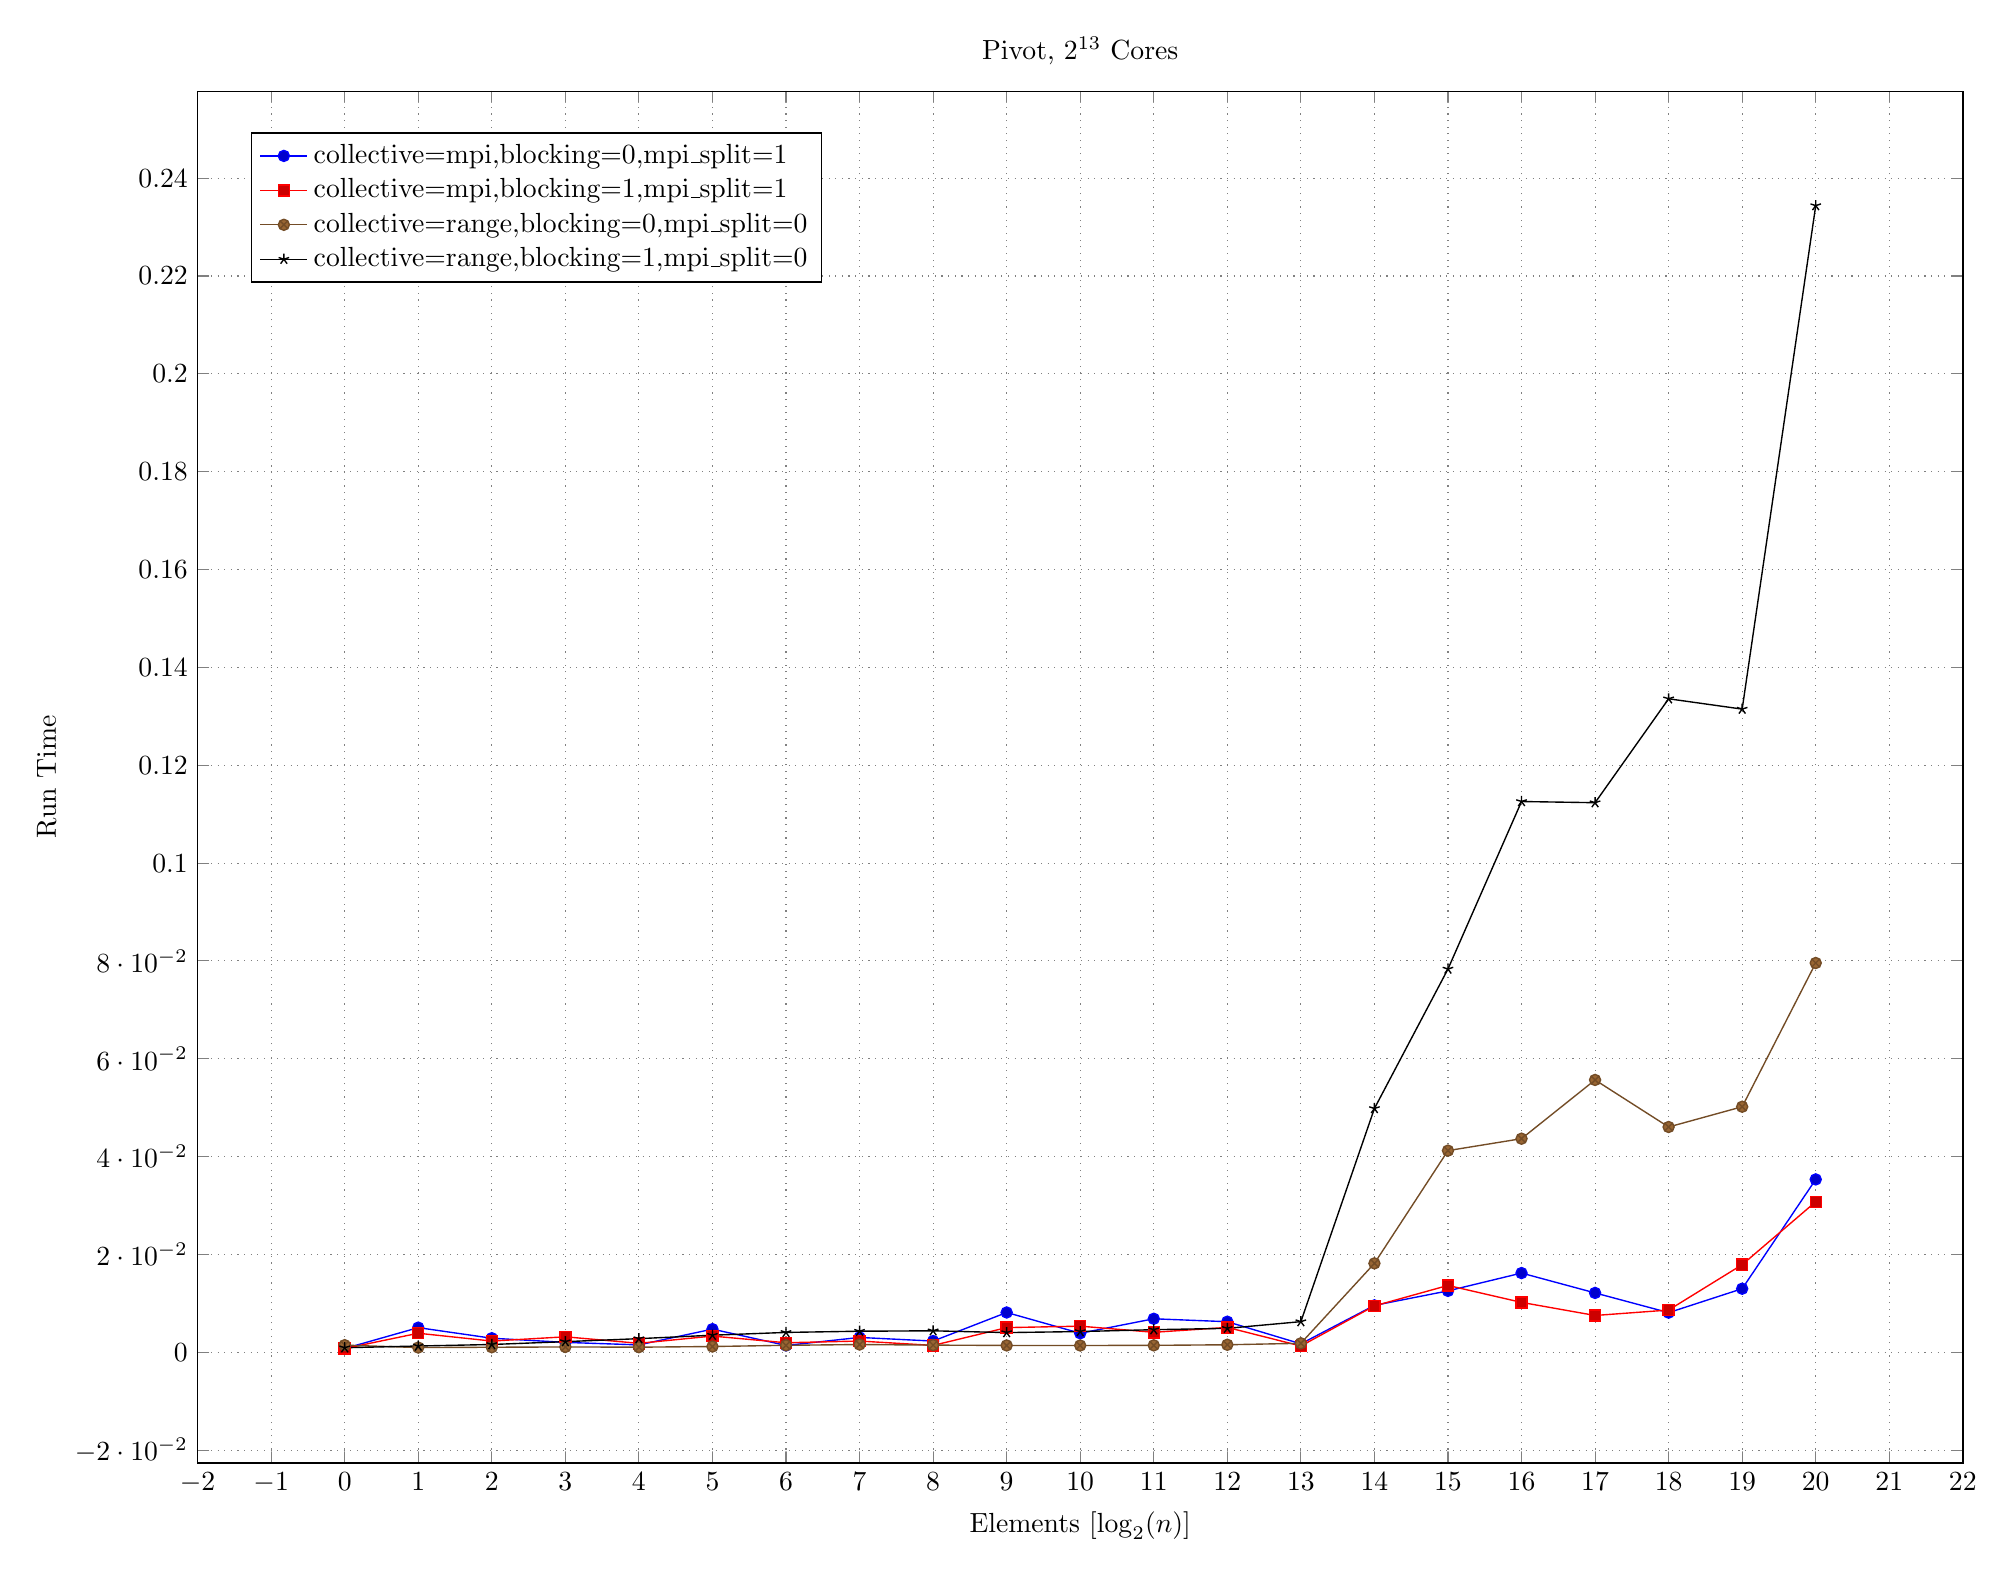
\begin{tikzpicture}
  \begin{axis}[
    title={Pivot, $2^{13}$ Cores},
    xlabel={Elements [$\log_2(n)$]},
    ylabel={Run Time},
    ]   
	%% MULTIPLOT(collective, blocking, mpi_split) SELECT LOG(2,elements) AS x, MEDIAN(pivot) as y, MULTIPLOT
	%% FROM ResultsQS
	%% WHERE size=8192
	%% GROUP BY MULTIPLOT, x  ORDER BY MULTIPLOT, x
 \addplot coordinates { (0.0,0.000771912) (1.0,0.00504151) (2.0,0.0028779) (3.0,0.00202444) (4.0,0.00151494) (5.0,0.00473435) (6.0,0.00139949) (7.0,0.00303696) (8.0,0.00229548) (9.0,0.00813985) (10.0,0.00389108) (11.0,0.00685096) (12.0,0.006254) (13.0,0.00173091) (14.0,0.00958919) (15.0,0.0125544) (16.0,0.0161958) (17.0,0.0121358) (18.0,0.0081053) (19.0,0.0129987) (20.0,0.0353393) };
 \addlegendentry{collective=mpi,blocking=0,mpi\_split=1};
 \addplot coordinates { (0.0,0.000765521) (1.0,0.00389629) (2.0,0.00229669) (3.0,0.003166) (4.0,0.00183602) (5.0,0.00331473) (6.0,0.00195113) (7.0,0.00230214) (8.0,0.00140612) (9.0,0.00504653) (10.0,0.00534177) (11.0,0.00408938) (12.0,0.00508616) (13.0,0.00128495) (14.0,0.00948411) (15.0,0.0136675) (16.0,0.0102017) (17.0,0.00752716) (18.0,0.00863708) (19.0,0.0179115) (20.0,0.0307753) };
 \addlegendentry{collective=mpi,blocking=1,mpi\_split=1};
 \addplot coordinates { (0.0,0.0014627) (1.0,0.000971664) (2.0,0.00103241) (3.0,0.00109449) (4.0,0.00104678) (5.0,0.00118117) (6.0,0.00142813) (7.0,0.00158903) (8.0,0.00146751) (9.0,0.00140237) (10.0,0.0013908) (11.0,0.00142024) (12.0,0.00153975) (13.0,0.00184019) (14.0,0.0181775) (15.0,0.0412252) (16.0,0.0436652) (17.0,0.0556712) (18.0,0.0460545) (19.0,0.050195) (20.0,0.0795779) };
 \addlegendentry{collective=range,blocking=0,mpi\_split=0};
 \addplot coordinates { (0.0,0.000932524) (1.0,0.00128649) (2.0,0.00159506) (3.0,0.00217718) (4.0,0.00278902) (5.0,0.00349469) (6.0,0.00406243) (7.0,0.00431068) (8.0,0.00439276) (9.0,0.00402786) (10.0,0.00424047) (11.0,0.0046232) (12.0,0.00489604) (13.0,0.0062676) (14.0,0.0498355) (15.0,0.0783477) (16.0,0.112587) (17.0,0.112344) (18.0,0.133585) (19.0,0.131476) (20.0,0.234395) };
 \addlegendentry{collective=range,blocking=1,mpi\_split=0};


  \end{axis}
\end{tikzpicture}
\newpage

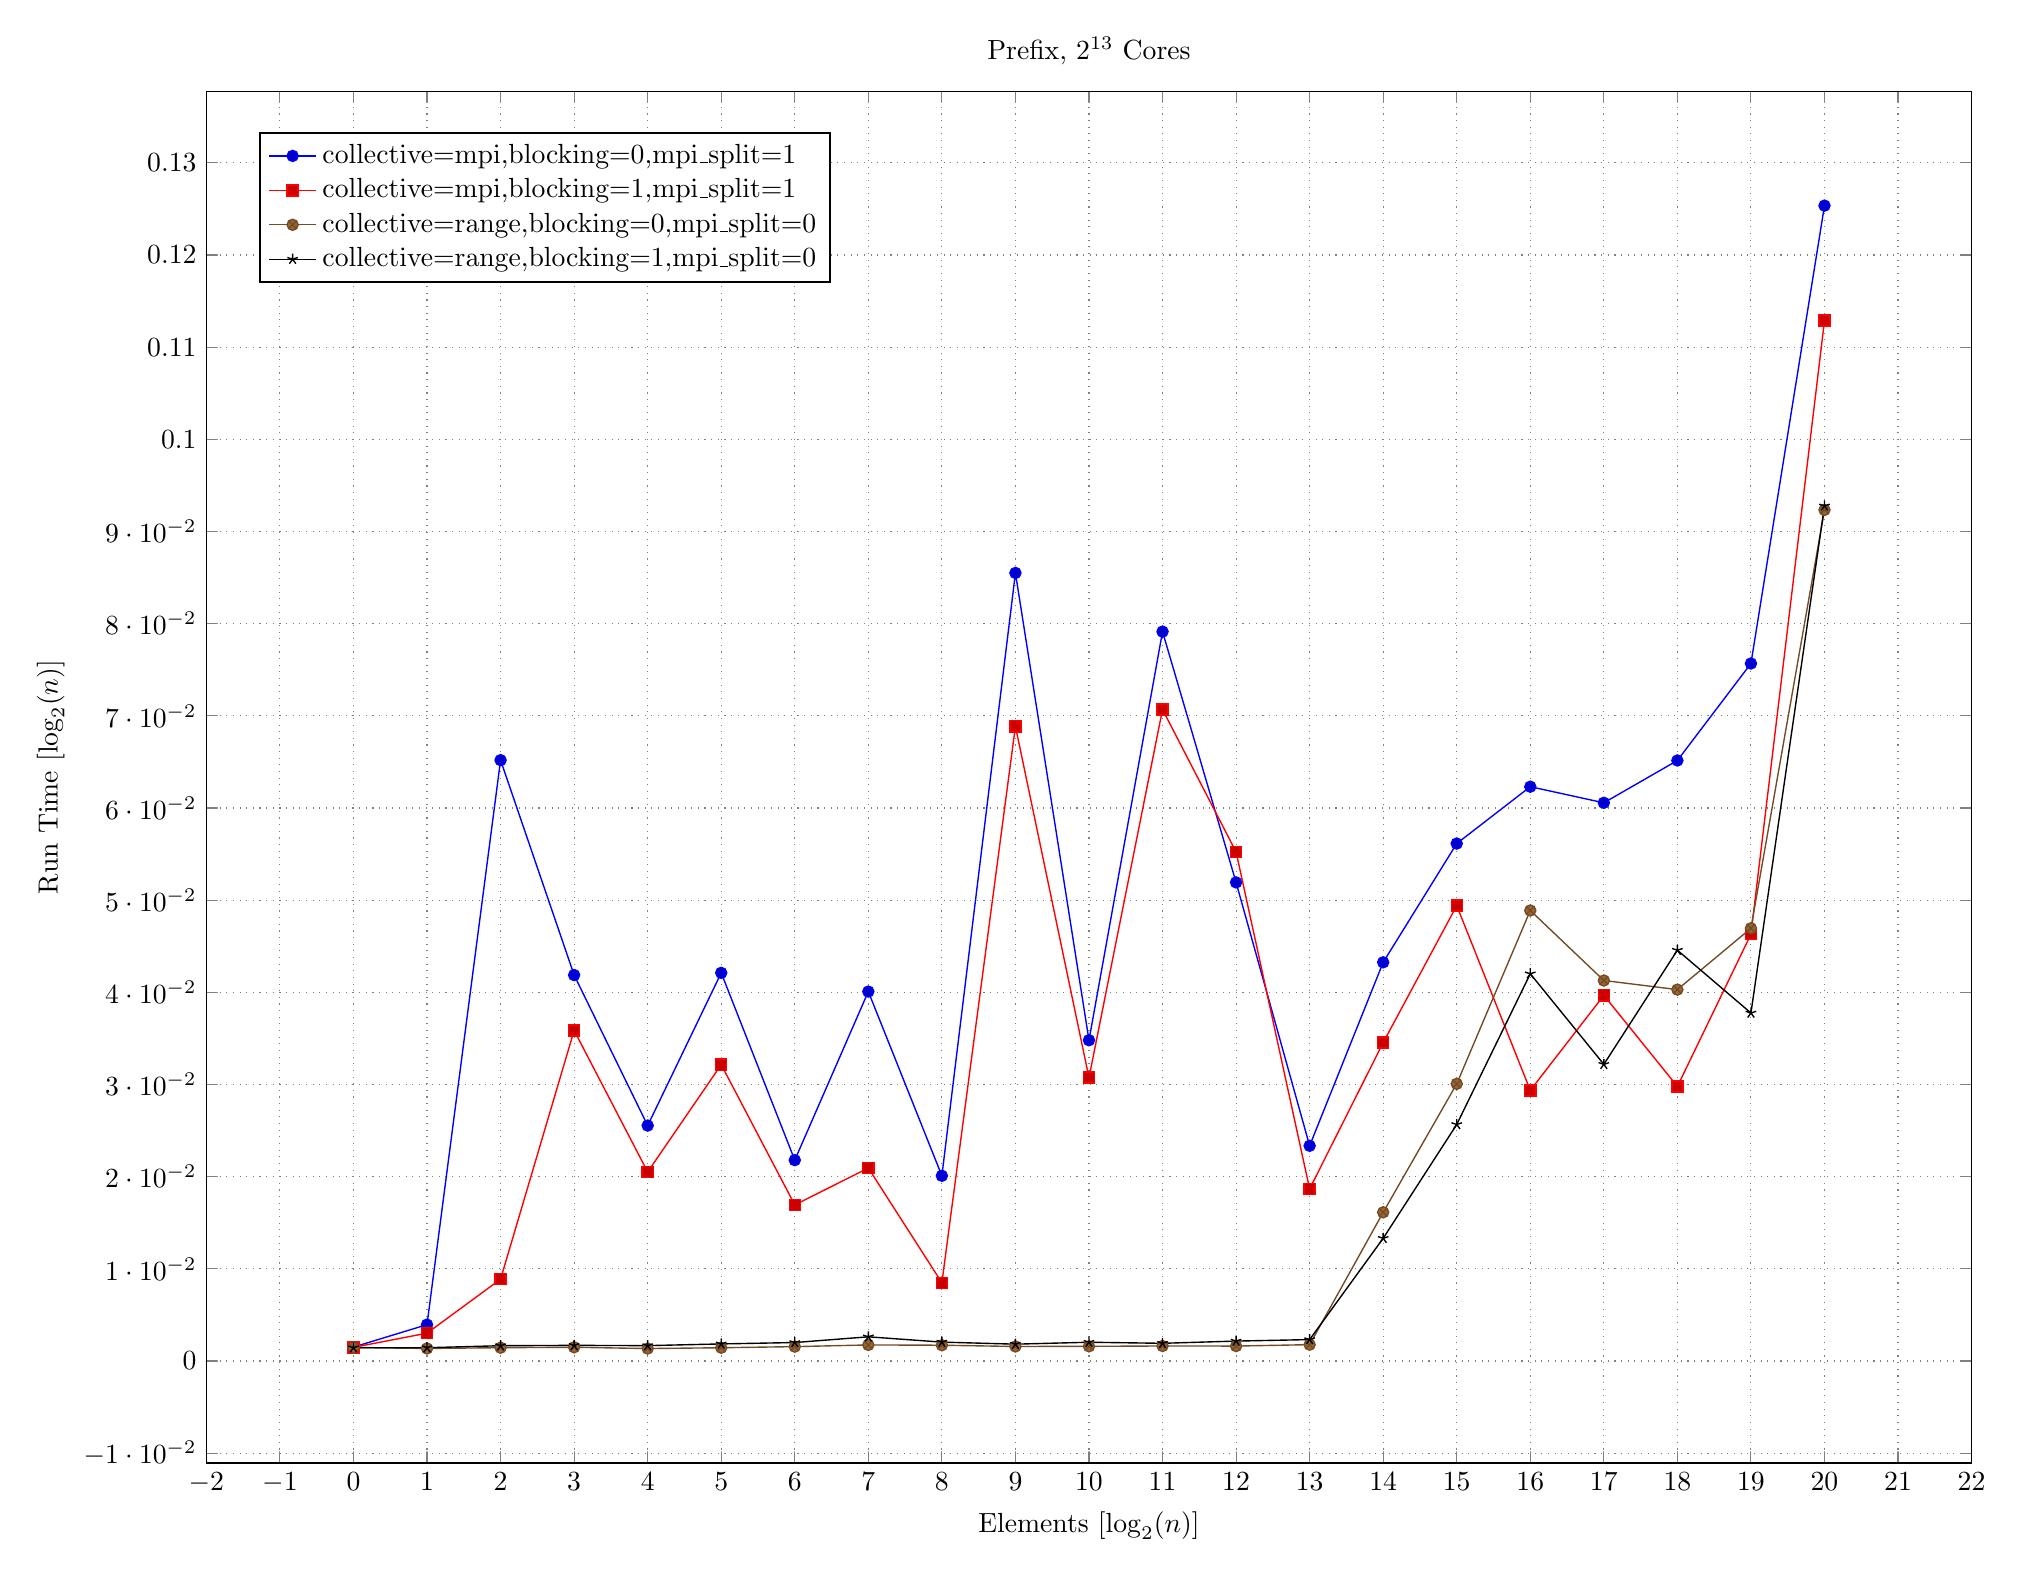
\begin{tikzpicture}
  \begin{axis}[
    title={Prefix, $2^{13}$ Cores},
    xlabel={Elements [$\log_2(n)$]},
    ylabel={Run Time [$\log_2(n)$]},
    ]   
	%% MULTIPLOT(collective, blocking, mpi_split) SELECT LOG(2,elements) AS x, MEDIAN(calculate) as y, MULTIPLOT
	%% FROM ResultsQS
	%% WHERE size=8192
	%% GROUP BY MULTIPLOT, x  ORDER BY MULTIPLOT, x
 \addplot coordinates { (0.0,0.00151158) (1.0,0.00394662) (2.0,0.0651932) (3.0,0.041876) (4.0,0.0255461) (5.0,0.0421162) (6.0,0.0217944) (7.0,0.0400856) (8.0,0.0200977) (9.0,0.0855035) (10.0,0.0348062) (11.0,0.0791382) (12.0,0.0519271) (13.0,0.0233523) (14.0,0.0432592) (15.0,0.0561435) (16.0,0.0623129) (17.0,0.0605645) (18.0,0.0651564) (19.0,0.0756798) (20.0,0.125358) };
 \addlegendentry{collective=mpi,blocking=0,mpi\_split=1};
 \addplot coordinates { (0.0,0.00148114) (1.0,0.00302294) (2.0,0.00887804) (3.0,0.0358656) (4.0,0.0205125) (5.0,0.0321547) (6.0,0.0169375) (7.0,0.0209417) (8.0,0.00849416) (9.0,0.0688629) (10.0,0.0307467) (11.0,0.0706867) (12.0,0.0552354) (13.0,0.018669) (14.0,0.03455) (15.0,0.0494081) (16.0,0.0293653) (17.0,0.0396763) (18.0,0.0297898) (19.0,0.0463049) (20.0,0.112883) };
 \addlegendentry{collective=mpi,blocking=1,mpi\_split=1};
 \addplot coordinates { (0.0,0.00146162) (1.0,0.00136357) (2.0,0.00144463) (3.0,0.0014914) (4.0,0.00135311) (5.0,0.0014415) (6.0,0.00156059) (7.0,0.00174545) (8.0,0.00171351) (9.0,0.00157745) (10.0,0.00159248) (11.0,0.00163117) (12.0,0.00162188) (13.0,0.00177552) (14.0,0.0161341) (15.0,0.0300761) (16.0,0.0488832) (17.0,0.0412846) (18.0,0.0402985) (19.0,0.0469523) (20.0,0.0923424) };
 \addlegendentry{collective=range,blocking=0,mpi\_split=0};
 \addplot coordinates { (0.0,0.00143606) (1.0,0.0014426) (2.0,0.00166103) (3.0,0.0016987) (4.0,0.00167045) (5.0,0.00185454) (6.0,0.0020063) (7.0,0.00262614) (8.0,0.00205196) (9.0,0.00182891) (10.0,0.00203776) (11.0,0.00192223) (12.0,0.00216329) (13.0,0.00232507) (14.0,0.0133151) (15.0,0.0256636) (16.0,0.0420157) (17.0,0.0321886) (18.0,0.0445731) (19.0,0.0377588) (20.0,0.0927796) };
 \addlegendentry{collective=range,blocking=1,mpi\_split=0};


  \end{axis}
\end{tikzpicture}
\newpage

\begin{tikzpicture}
  \begin{axis}[
    title={Sum, $2^{13}$ Cores},
    xlabel={Elements [$\log_2(n)$]},
    ylabel={Run Time [$\log_2(n)$]},
    ]   
	%% PLOT SELECT LOG(2,elements) AS x, LOG(2,MIN(runtime)) as y
	%% FROM ResultsQS
	%% WHERE size=8192 AND collective="range" AND blocking=0 AND mpi_split=0
	%% GROUP BY x  ORDER BY x
 \addplot coordinates { (0.0,-6.51823) (1.0,-6.90689) (2.0,-6.73866) (3.0,-6.73131) (4.0,-6.85184) (5.0,-6.71338) (6.0,-6.55519) (7.0,-6.40474) (8.0,-6.42083) (9.0,-6.36073) (10.0,-6.26958) (11.0,-6.27741) (12.0,-5.97903) (13.0,-5.50666) (14.0,-2.54635) (15.0,-1.96727) (16.0,-1.66535) (17.0,-1.70275) (18.0,-1.00519) (19.0,-0.166449) (20.0,0.869903) };
	
	%% PLOT SELECT LOG(2,elements) AS x, LOG(2,MAX(runtime)) as y
	%% FROM ResultsQS
	%% WHERE size=8192 AND collective="range" AND blocking=0 AND mpi_split=0
	%% GROUP BY x  ORDER BY x
 \addplot coordinates { (0.0,-5.34115) (1.0,-6.63112) (2.0,-6.46917) (3.0,-6.3779) (4.0,-6.36541) (5.0,-6.39458) (6.0,-6.25358) (7.0,-5.66298) (8.0,-6.08772) (9.0,-6.02084) (10.0,-6.00491) (11.0,-5.86158) (12.0,-5.6416) (13.0,-5.14367) (14.0,-2.05841) (15.0,-1.43321) (16.0,-1.24124) (17.0,-0.904845) (18.0,-0.713746) (19.0,0.0264177) (20.0,1.17673) };


  \end{axis}
\end{tikzpicture}
\newpage

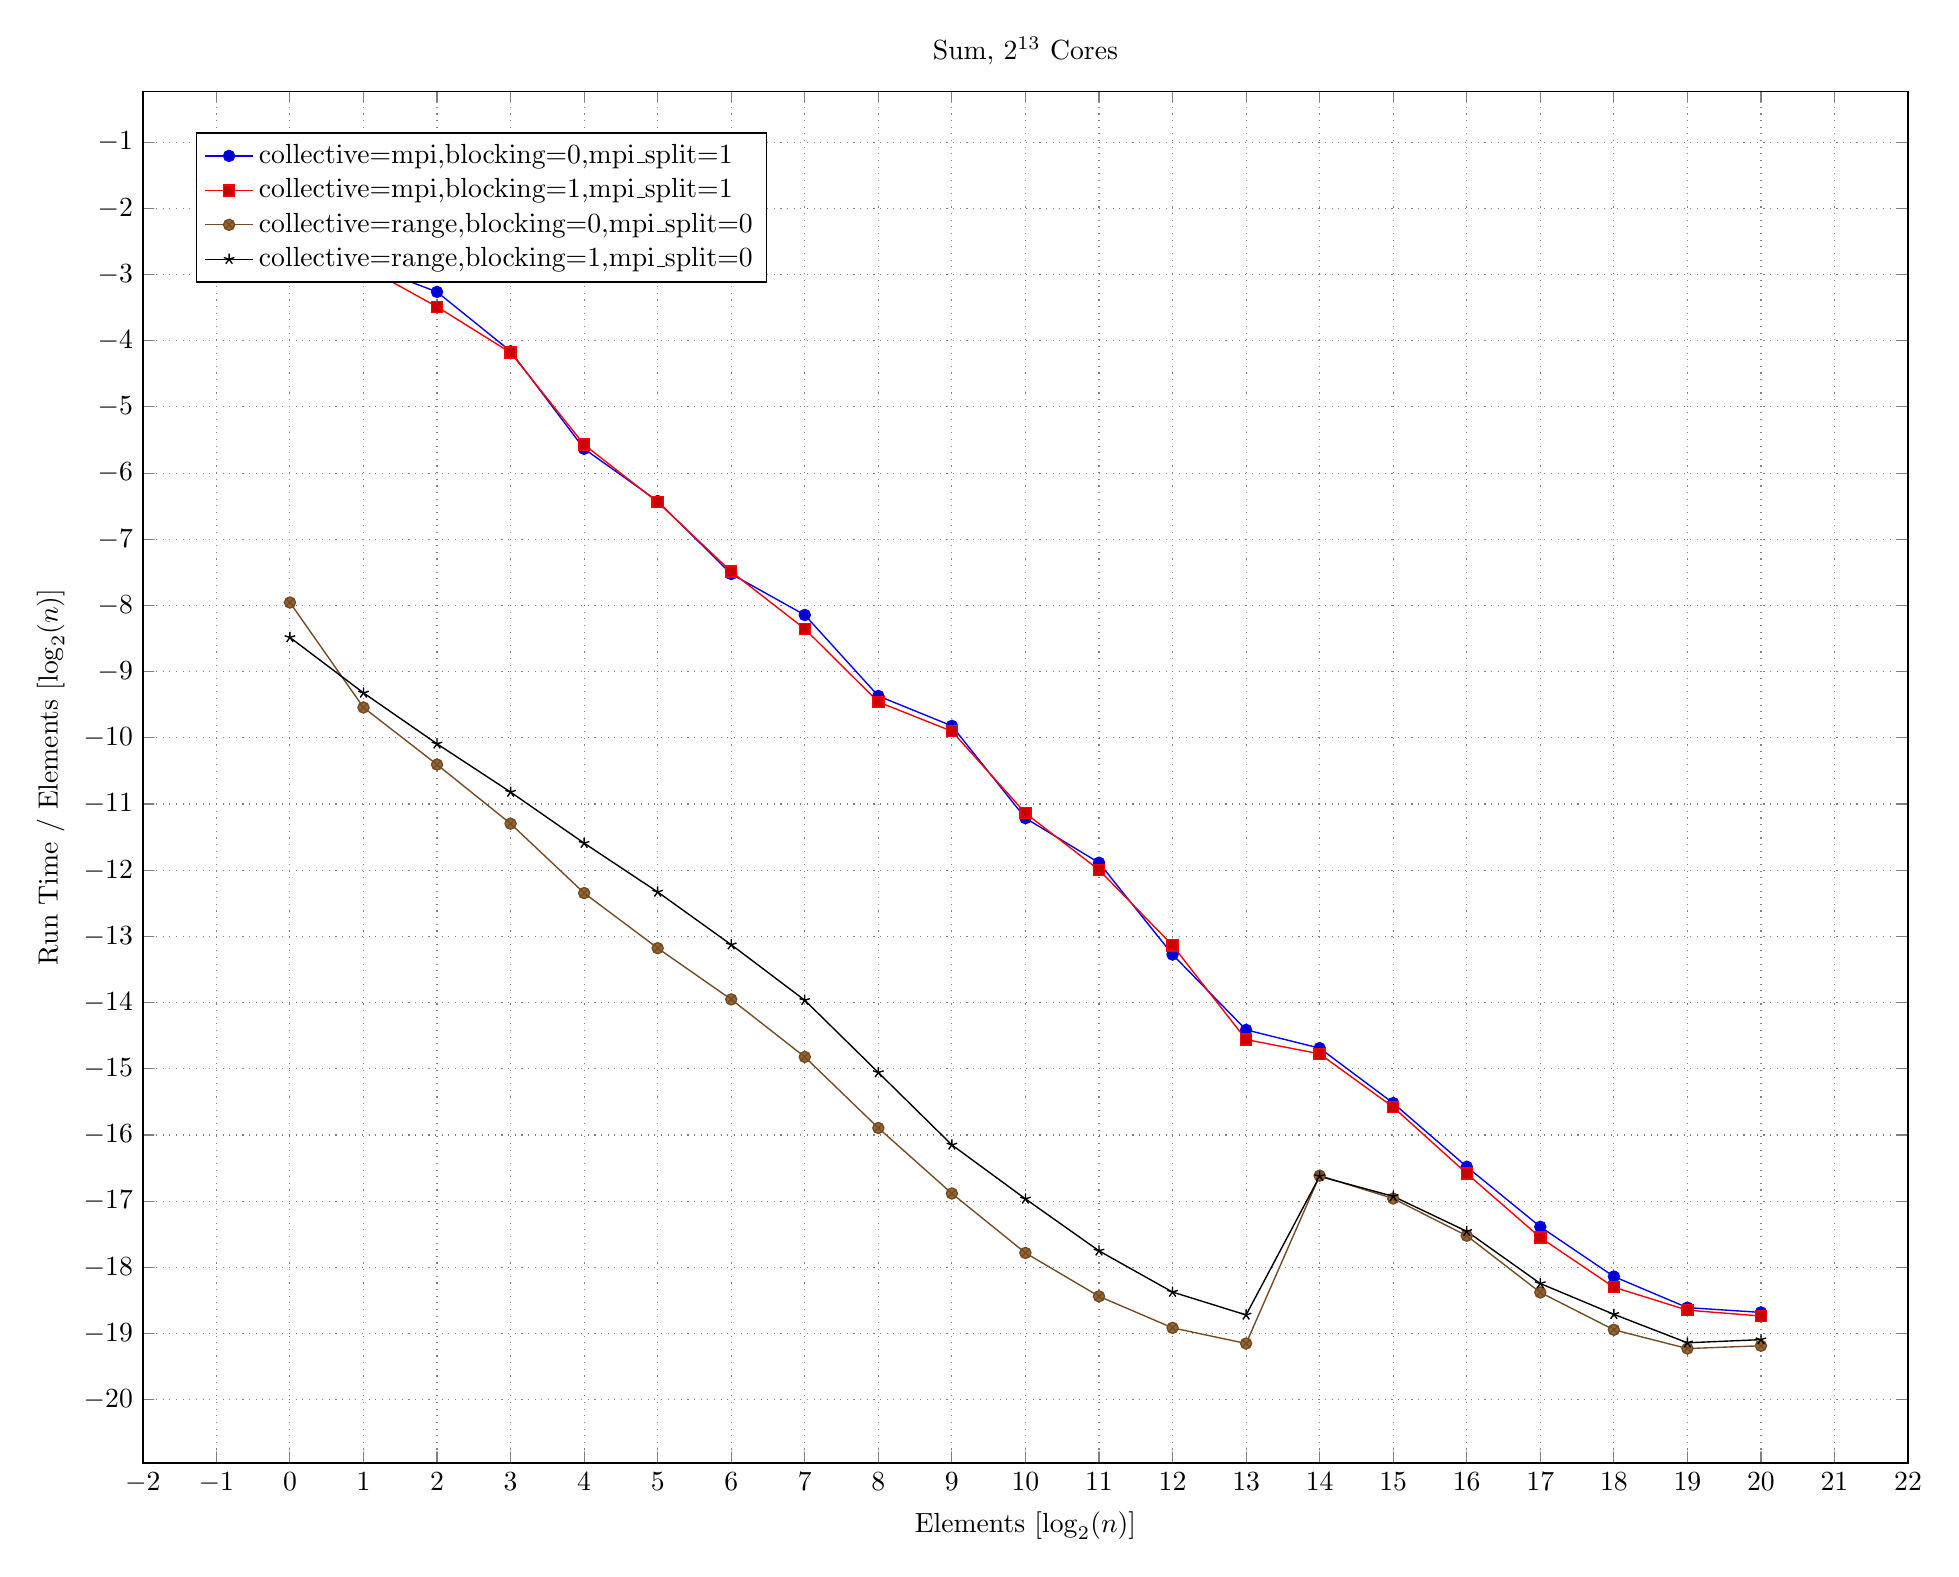
\begin{tikzpicture}
  \begin{axis}[
    title={Sum, $2^{13}$ Cores},
    xlabel={Elements [$\log_2(n)$]},
    ylabel={Run Time / Elements [$\log_2(n)$]},
    ]   
	%% MULTIPLOT(collective, blocking, mpi_split) SELECT LOG(2,elements) AS x, LOG(2,MEDIAN(sum)/elements) as y, MULTIPLOT
	%% FROM ResultsQS
	%% WHERE size=8192
	%% GROUP BY MULTIPLOT, x  ORDER BY MULTIPLOT, x
 \addplot coordinates { (0.0,-2.0907) (1.0,-2.83892) (2.0,-3.2623) (3.0,-4.15858) (4.0,-5.63234) (5.0,-6.42269) (6.0,-7.52382) (7.0,-8.14318) (8.0,-9.36726) (9.0,-9.81887) (10.0,-11.2132) (11.0,-11.8867) (12.0,-13.2739) (13.0,-14.4118) (14.0,-14.6878) (15.0,-15.5185) (16.0,-16.4802) (17.0,-17.3874) (18.0,-18.1389) (19.0,-18.6088) (20.0,-18.6808) };
 \addlegendentry{collective=mpi,blocking=0,mpi\_split=1};
 \addplot coordinates { (0.0,-1.95796) (1.0,-2.87184) (2.0,-3.4868) (3.0,-4.17868) (4.0,-5.56966) (5.0,-6.43799) (6.0,-7.48853) (7.0,-8.35319) (8.0,-9.45756) (9.0,-9.8998) (10.0,-11.1377) (11.0,-11.9954) (12.0,-13.1345) (13.0,-14.5585) (14.0,-14.7744) (15.0,-15.5791) (16.0,-16.5819) (17.0,-17.5503) (18.0,-18.3) (19.0,-18.647) (20.0,-18.7357) };
 \addlegendentry{collective=mpi,blocking=1,mpi\_split=1};
 \addplot coordinates { (0.0,-7.95495) (1.0,-9.54132) (2.0,-10.4036) (3.0,-11.2964) (4.0,-12.345) (5.0,-13.1776) (6.0,-13.9519) (7.0,-14.8209) (8.0,-15.8944) (9.0,-16.8843) (10.0,-17.7825) (11.0,-18.438) (12.0,-18.9145) (13.0,-19.1507) (14.0,-16.6145) (15.0,-16.9607) (16.0,-17.5226) (17.0,-18.3796) (18.0,-18.9439) (19.0,-19.2271) (20.0,-19.1852) };
 \addlegendentry{collective=range,blocking=0,mpi\_split=0};
 \addplot coordinates { (0.0,-8.48248) (1.0,-9.32101) (2.0,-10.0904) (3.0,-10.8193) (4.0,-11.5912) (5.0,-12.3289) (6.0,-13.1259) (7.0,-13.9647) (8.0,-15.0567) (9.0,-16.1505) (10.0,-16.9658) (11.0,-17.7513) (12.0,-18.3738) (13.0,-18.7193) (14.0,-16.6256) (15.0,-16.9269) (16.0,-17.456) (17.0,-18.2447) (18.0,-18.7098) (19.0,-19.1402) (20.0,-19.0924) };
 \addlegendentry{collective=range,blocking=1,mpi\_split=0};


  \end{axis}
\end{tikzpicture}
\newpage

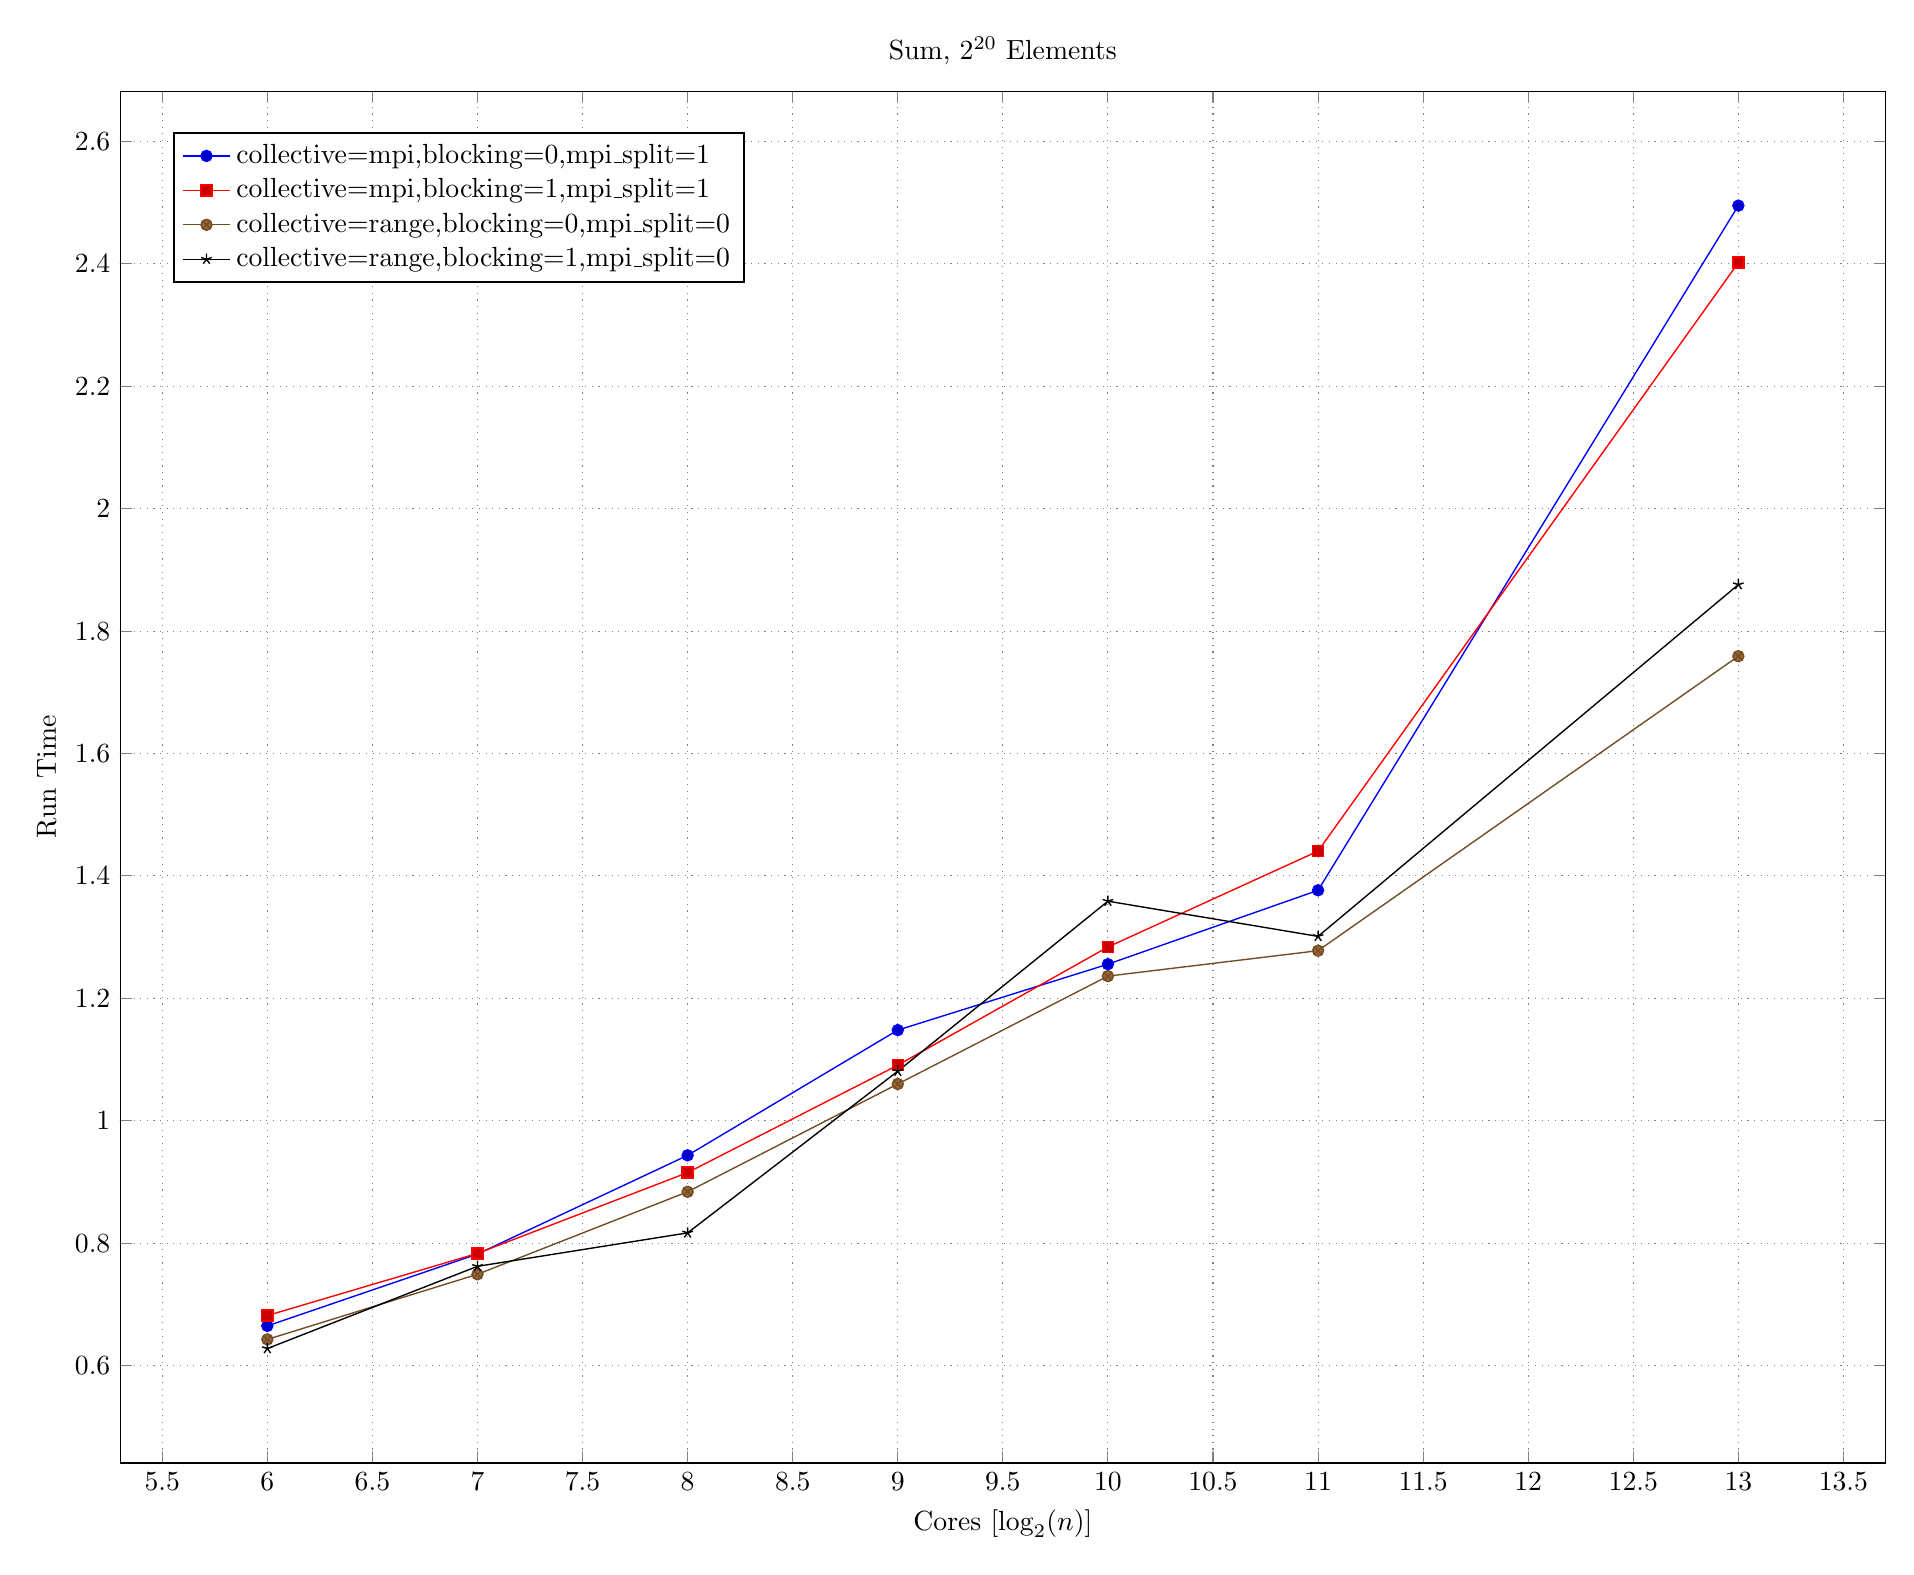
\begin{tikzpicture}
  \begin{axis}[
    title={Sum, $2^{20}$ Elements},
    xlabel={Cores [$\log_2(n)$]},
    ylabel={Run Time},
    ]   
	%% MULTIPLOT(collective, blocking, mpi_split) SELECT LOG(2,size) AS x, MEDIAN(sum) as y, MULTIPLOT
	%% FROM ResultsQS
	%% WHERE elements=POWER(2,20)
	%% GROUP BY MULTIPLOT, x  ORDER BY MULTIPLOT, x
 \addplot coordinates { (6.0,0.664772) (7.0,0.782177) (8.0,0.943454) (9.0,1.14808) (10.0,1.25577) (11.0,1.37653) (13.0,2.495235) };
 \addlegendentry{collective=mpi,blocking=0,mpi\_split=1};
 \addplot coordinates { (6.0,0.681663) (7.0,0.783262) (8.0,0.915271) (9.0,1.09078) (10.0,1.28385) (11.0,1.44054) (13.0,2.402035) };
 \addlegendentry{collective=mpi,blocking=1,mpi\_split=1};
 \addplot coordinates { (6.0,0.642666) (7.0,0.749107) (8.0,0.883892) (9.0,1.06003) (10.0,1.23629) (11.0,1.27784) (13.0,1.759015) };
 \addlegendentry{collective=range,blocking=0,mpi\_split=0};
 \addplot coordinates { (6.0,0.627767) (7.0,0.762116) (8.0,0.816757) (9.0,1.08092) (10.0,1.35873) (11.0,1.30121) (13.0,1.875925) };
 \addlegendentry{collective=range,blocking=1,mpi\_split=0};


  \end{axis}
\end{tikzpicture}
\newpage

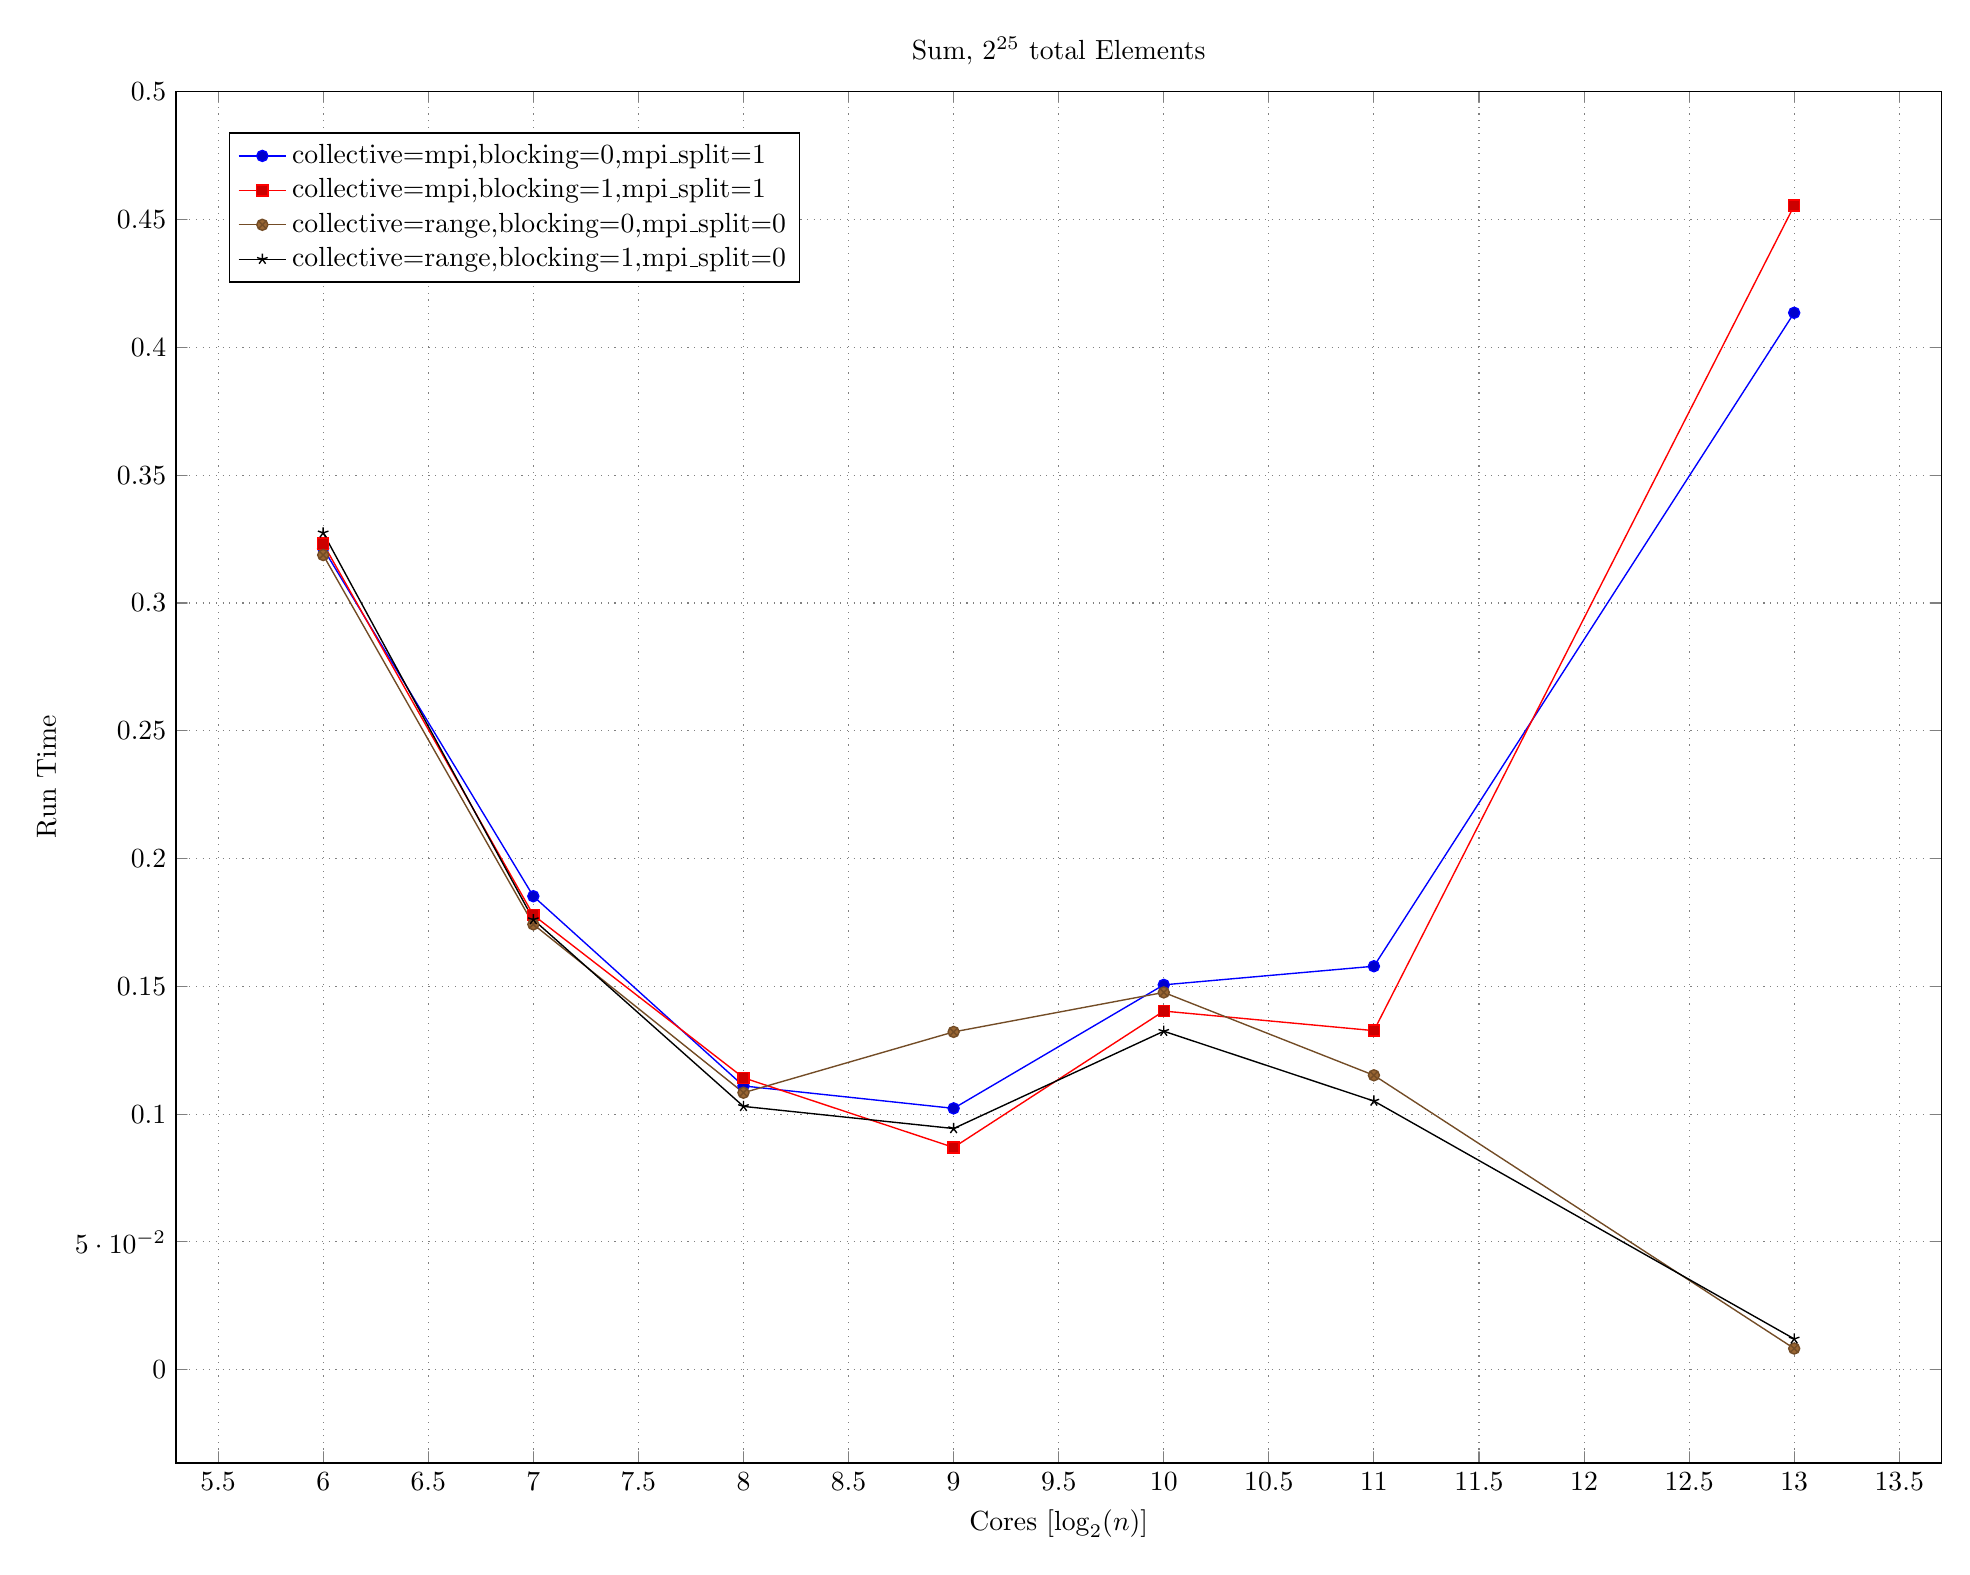
\begin{tikzpicture}
  \begin{axis}[
    title={Sum, $2^{25}$ total Elements},
    xlabel={Cores [$\log_2(n)$]},
    ylabel={Run Time},
    ]   
	%% MULTIPLOT(collective, blocking, mpi_split) SELECT LOG(2,size) AS x, MEDIAN(sum) as y, MULTIPLOT
	%% FROM ResultsQS
	%% WHERE elements*size=POWER(2,25)
	%% GROUP BY MULTIPLOT, x  ORDER BY MULTIPLOT, x
 \addplot coordinates { (6.0,0.321367) (7.0,0.185262) (8.0,0.11103) (9.0,0.102263) (10.0,0.150594) (11.0,0.157871) (13.0,0.413542) };
 \addlegendentry{collective=mpi,blocking=0,mpi\_split=1};
 \addplot coordinates { (6.0,0.323199) (7.0,0.1779) (8.0,0.114238) (9.0,0.0869758) (10.0,0.140331) (11.0,0.132673) (13.0,0.455477) };
 \addlegendentry{collective=mpi,blocking=1,mpi\_split=1};
 \addplot coordinates { (6.0,0.318766) (7.0,0.174255) (8.0,0.108382) (9.0,0.132176) (10.0,0.147622) (11.0,0.1152) (13.0,0.00828929) };
 \addlegendentry{collective=range,blocking=0,mpi\_split=0};
 \addplot coordinates { (6.0,0.327448) (7.0,0.17613) (8.0,0.103031) (9.0,0.0943719) (10.0,0.132443) (11.0,0.105132) (13.0,0.0120582) };
 \addlegendentry{collective=range,blocking=1,mpi\_split=0};


  \end{axis}
\end{tikzpicture}
\newpage
%
%\begin{tikzpicture}
%  \begin{axis}[
%    title={Range, $2^{20}$ elements},
%    xlabel={Cores [$\log_2(n)$]},
%    ylabel={Run Time},
%    ]   
%	%% MULTIPLOT(Type) SELECT elements, collective, LOG(2,size) AS x, Time as y, MULTIPLOT FROM (    
%	%% SELECT elements, size, MEDIAN(pivot) as Time, 'Pivot' as Type, collective, blocking, mpi_split
%	%% FROM ResultsQS
%	%% GROUP BY collective, size, elements, blocking, mpi_split
%	%% UNION ALL
%	%% SELECT elements, size, MEDIAN(partition) as Time, 'Partition' as Type, collective, blocking, mpi_split
%	%% FROM ResultsQS
%	%% GROUP BY collective, size, elements, blocking, mpi_split
%	%% UNION ALL
%	%% SELECT elements, size, MEDIAN(calculate) as Time, 'Prefix' as Type, collective, blocking, mpi_split
%	%% FROM ResultsQS
%	%% GROUP BY collective, size, elements, blocking, mpi_split
%	%% UNION ALL
%	%% SELECT elements, size, MEDIAN(exchange) as Time, 'Exchange' as Type, collective, blocking, mpi_split
%	%% FROM ResultsQS
%	%% GROUP BY collective, size, elements, blocking, mpi_split
%	%% UNION ALL
%	%% SELECT elements, size, MEDIAN(create_comms) as Time, 'Create Comms' as Type, collective, blocking, mpi_split
%	%% FROM ResultsQS
%	%% GROUP BY collective, size, elements, blocking, mpi_split
%	%% UNION ALL
%	%% SELECT elements, size, MEDIAN(sort_two) as Time, 'Sort on 2' as Type, collective, blocking, mpi_split
%	%% FROM ResultsQS
%	%% GROUP BY collective, size, elements, blocking, mpi_split
%	%% UNION ALL
%	%% SELECT elements, size, MEDIAN(sort_local) as Time, 'Sort local' as Type, collective, blocking, mpi_split
%	%% FROM ResultsQS
%	%% GROUP BY collective, size, elements, blocking, mpi_split
%	%% ) a
%	%% WHERE collective="mpi" AND elements=POWER(2,20) AND blocking=1 AND mpi_split=1
%	%% GROUP BY MULTIPLOT, x  ORDER BY MULTIPLOT, x
% \addplot coordinates { (9.0,0.28771) (10.0,0.288046) (12.0,0.560685) (13.0,0.788634) };
% \addlegendentry{Type=Create Comms};
% \addplot coordinates { (9.0,0.780469) (10.0,0.893874) (12.0,1.48837) (13.0,1.58243) };
% \addlegendentry{Type=Exchange};
% \addplot coordinates { (9.0,0.358772) (10.0,0.402246) (12.0,0.514516) (13.0,0.540983) };
% \addlegendentry{Type=Partition};
% \addplot coordinates { (9.0,0.0774949) (10.0,0.0483513) (12.0,0.0597702) (13.0,0.0625685) };
% \addlegendentry{Type=Pivot};
% \addplot coordinates { (9.0,0.0544872) (10.0,0.054643) (12.0,0.0933107) (13.0,0.103632) };
% \addlegendentry{Type=Prefix};
% \addplot coordinates { (9.0,0.366853) (10.0,0.38417) (12.0,0.394019) (13.0,0.396668) };
% \addlegendentry{Type=Sort local};
% \addplot coordinates { (9.0,1.27432) (10.0,1.30545) (12.0,1.32591) (13.0,1.33269) };
% \addlegendentry{Type=Sort on 2};
%
%
%  \end{axis}
%\end{tikzpicture}
%\newpage

%\begin{tikzpicture}
%\begin{axis}[
%title={Pivot, $2^{20}$ elements},
%xlabel={Cores [$\log_2(n)$]},
%ylabel={Run Time},
%]   
% %% MULTIPLOT(Type) SELECT elements, LOG(2,size) AS x, Time as y, MULTIPLOT FROM (    
% %% SELECT elements, size, MEDIAN(pivot) as Time, 'Range' as Type
% %% FROM ResultsQS
% %% WHERE collective="range" AND blocking=0 AND mpi_split=0
% %% GROUP BY size, elements
% %% UNION ALL
% %% SELECT elements, size, MEDIAN(pivot) as Time, 'Range blocking' as Type
% %% FROM ResultsQS
% %% WHERE collective="range" AND blocking=1 AND mpi_split=0
% %% GROUP BY size, elements
% %% UNION ALL
% %% SELECT elements, size, MEDIAN(pivot) as Time, 'Range mpi_split' as Type
% %% FROM ResultsQS
% %% WHERE collective="range" AND blocking=0 AND mpi_split=1
% %% GROUP BY size, elements
% %% UNION ALL
% %% SELECT elements, size, MEDIAN(pivot) as Time, 'MPI blocking' as Type
% %% FROM ResultsQS
% %% WHERE collective="mpi" AND blocking=1 AND mpi_split=1
% %% GROUP BY size, elements
% %% ) a
% %% WHERE elements=POWER(2,20)
% %% GROUP BY MULTIPLOT, x  ORDER BY MULTIPLOT, x
%\addplot coordinates { (9.0,0.0774949) (10.0,0.0483513) (12.0,0.0597702) (13.0,0.0625685) };
%\addlegendentry{Type=MPI blocking};
%\addplot coordinates { (9.0,0.125294) (10.0,0.123921) (12.0,0.146194) (13.0,0.151579) };
%\addlegendentry{Type=Range};
%\addplot coordinates { (9.0,0.223502) (10.0,0.195748) (12.0,0.291215) (13.0,0.398244) };
%\addlegendentry{Type=Range blocking};
%\addplot coordinates { (9.0,0.0172105) (10.0,0.0280767) (12.0,0.0579143) (13.0,0.0791711) };
%\addlegendentry{Type=Range mpi\_split};
%
%
%\end{axis}
%\end{tikzpicture}
%\newpage
%
%\begin{tikzpicture}
%\begin{axis}[
%title={Prefix sum, $2^{20}$ elements},
%xlabel={Cores [$\log_2(n)$]},
%ylabel={Run Time},
%]   
% %% MULTIPLOT(Type) SELECT elements, LOG(2,size) AS x, Time as y, MULTIPLOT FROM (    
% %% SELECT elements, size, MEDIAN(calculate) as Time, 'Range' as Type
% %% FROM ResultsQS
% %% WHERE collective="range" AND blocking=0 AND mpi_split=0
% %% GROUP BY size, elements
% %% UNION ALL
% %% SELECT elements, size, MEDIAN(calculate) as Time, 'Range blocking' as Type
% %% FROM ResultsQS
% %% WHERE collective="range" AND blocking=1 AND mpi_split=0
% %% GROUP BY size, elements
% %% UNION ALL
% %% SELECT elements, size, MEDIAN(calculate) as Time, 'Range mpi_split' as Type
% %% FROM ResultsQS
% %% WHERE collective="range" AND blocking=0 AND mpi_split=1
% %% GROUP BY size, elements
% %% UNION ALL
% %% SELECT elements, size, MEDIAN(calculate) as Time, 'MPI blocking' as Type
% %% FROM ResultsQS
% %% WHERE collective="mpi" AND blocking=1 AND mpi_split=1
% %% GROUP BY size, elements
% %% ) a
% %% WHERE elements=POWER(2,20)
% %% GROUP BY MULTIPLOT, x  ORDER BY MULTIPLOT, x
%\addplot coordinates { (9.0,0.0544872) (10.0,0.054643) (12.0,0.0933107) (13.0,0.103632) };
%\addlegendentry{Type=MPI blocking};
%\addplot coordinates { (9.0,0.0733838) (10.0,0.0860003) (12.0,0.134109) (13.0,0.145614) };
%\addlegendentry{Type=Range};
%\addplot coordinates { (9.0,0.0567608) (10.0,0.0705758) (12.0,0.0870146) (13.0,0.132569) };
%\addlegendentry{Type=Range blocking};
%\addplot coordinates { (9.0,0.0537762) (10.0,0.0647017) (12.0,0.11611) (13.0,0.125948) };
%\addlegendentry{Type=Range mpi\_split};
%
%
%\end{axis}
%\end{tikzpicture}
%\newpage

\end{center}

\end{document}

%%%%%%%%%%%%%%%%%%%%%%%%%%%%%%%%%%%%%%%%%%%%%%%%%%%%%%%%%%%%%%%%%%%%%%%%%%%%%%%%
